\documentclass{beamer}
\usepackage[british,spanish]{babel}
\usepackage[utf8]{inputenc}
\usepackage{hyperref}
\usepackage{multirow}



\usepackage{listings}

\usepackage{adjustbox}
\usepackage{lstcustom}

\usepackage{color}
\definecolor{light-gray}{gray}{0.80}
\definecolor{lstbackgroundshellcolor}{named}{light-gray}

\usepackage{tikz}
\newcommand*\circled[1]{\tikz[baseline=(char.base)]{
            \node[shape=circle,draw,inner sep=2pt] (char) {#1};}}

\usepackage[normalem]{ulem}

%\usepackage[acronym,xindy,toc]{glossaries}

\usepackage[acronym,xindy,toc]{glossaries}
\makeglossaries
%\usepackage[xindy]{imakeidx}
%\makeindex

\newcommand{\comment}[2]{#2}

\graphicspath{ {./images/} }

\title[Cloud Computing with Amazon Web Services]{Scaling with Amazon Web Services}
%\subtitle[short subtitle]{long subtitle}
\author[C. Cuenca, F. Quintana]{Carmelo Cuenca-Hernández and Francisca Quintana-Domínguez}
%\institute{Escuela Universitaria de Informática}
%\date[04/2013]{Abril - 2013}
\date{}
\titlegraphic{
\includegraphics[width=0.5 \textwidth]{images/awslogo.eps}}

\newcommand{\outputcommand}[1]{\color{darkgreen}{#1}}

\pgfdeclareimage[width=2.0\baselineskip]{ulpgc-logo}{images/logosimbolo_secundario_version_vertical}
\setbeamertemplate{footline}{\raisebox{-2ex}{\pgfuseimage{ulpgc-logo}}
  \usebeamerfont{date in head/foot}\insertshortdate{}\hfill
  \usebeamertemplate{navigation symbols}\hfill
  \insertframenumber{}/\inserttotalframenumber}
\setbeamertemplate{sidebar right}{}


\usetheme{Antibes}
%\usetheme{Berlin}

%\usetheme{Warsaw}
%\usecolortheme{albatross}

\begin{document}

\begin{frame}
	\titlepage
\end{frame}


\section*{Outline}
\begin{frame}[fragile, allowframebreaks]
  \frametitle{Outline}
  %\tableofcontents%[part=1,pausesections]
  %\tableofcontents[currentsection,currentsubsection, sectionstyle=show] 
  \tableofcontents[currentsection,sectionstyle=show,hideothersubsections]
\end{frame}


\selectlanguage{british}

%%%%%%%%%%%%%%%%%%%%%%%%%%%%%%%%%%%%%%%%%%%%%%%%%%%%%%%%%%%%%%%%%%%%%%%%%%%%%%
%\newacronym{<label>}{<abbrv>}{<full>}
%\glsreset{<label>}
%\glsresetall
%\acrlong{<label>}
%\acrfull{<label>}
%\acrshort{<label>}
\newacronym{ami}{AMI}{Amazon Machine Image}
\newacronym{aws}{AWS}{Amazon Web Services}
\newacronym{ebs}{EBS}{Elastic Block Storage}
\newacronym{ec2}{EC2}{Amazon Elastic Compute Cloud}
\newacronym{ecu}{ECU}{Elastic Compute Unit}
\newacronym{elb}{ELB}{Elastic Load Balancing}
\newacronym{rds}{RDS}{Relational Database Service}
\newacronym{s3}{S3}{Simple Storage Service}
\newacronym{sqs}{SQS}{Amazon Simple Queue Service}
%%%%%%%%%%%%%%%%%%%%%%%%%%%%%%%%%%%%%%%%%%%%%%%%%%%%%%%%%%%%%%%%%%%%%%%%%%%%%%
%%%%%%%%%%%%%%%%%%%%%%%%%%%%%%%%%%%%%%%%%%%%%%%%%%%%%%%%%%%%%%%%%%%%%%%%%%%%%%
\section{Scaling with Amazon Web Services}
\begin{frame}[fragile, allowframebreaks]
\frametitle{Scaling with Amazon Web Services}

\begin{columns}
\column{0.5 \textwidth}

\begin{center}
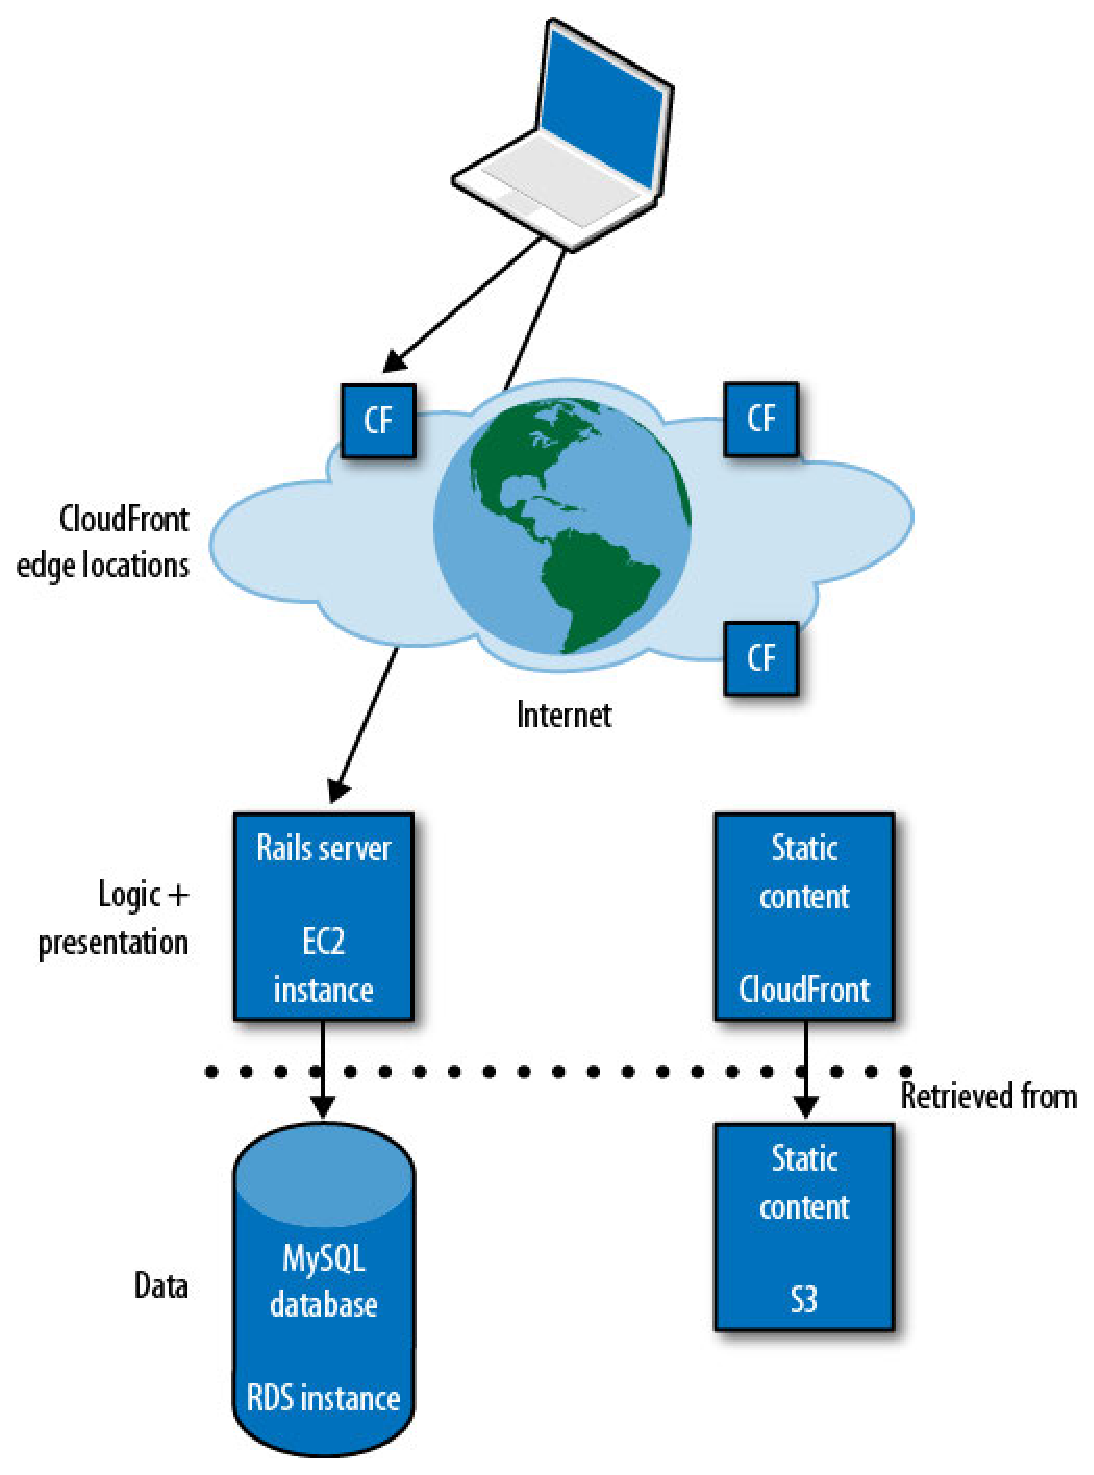
\includegraphics[scale=0.20]{Programming_Amazon_EC2-013.eps}      
\end{center}
\column{0.5 \textwidth}
\begin{center}
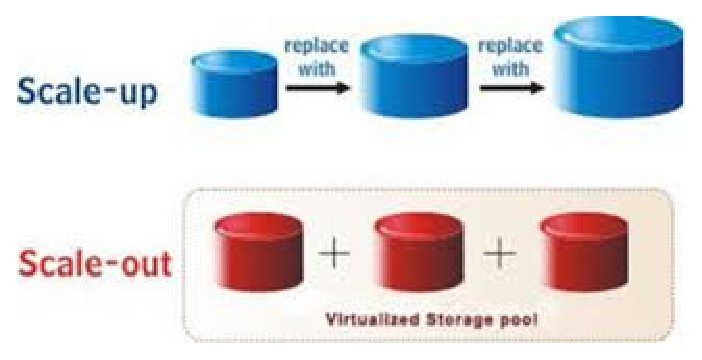
\includegraphics[scale=0.45]{scale.eps}
\end{center}
\end{columns}

\begin{itemize}
 \item We have a standard, three-tiered application, consisting of a database, an application server, and a web server
 \item Scaling considerations
 \begin{itemize}
   \item You cannot guarantee that the load balancer will redirect subsequents request from the same user to the same \acrshort{ec2} instance
   \item Ephemeral Filesystems. The current state of the filesystem can be assumed to last only as long a single resquest (File Uploads?)
   \item Embedded Databases store their data in a file on the local filesystem
   \item Caching (MemCache, REDIS \dots...)
   \item Storing Static Assets
 \end{itemize}
\end{itemize}


\end{frame}
%%%%%%%%%%%%%%%%%%%%%%%%%%%%%%%%%%%%%%%%%%%%%%%%%%%%%%%%%%%%%%%%%%%%%%%%%%%%%%
\section{RDS Database}
\begin{frame}[fragile, allowframebreaks]
\frametitle{RDS Database}
\begin{itemize}
 \item \acrfull{rds} is a web service that makes it easy to set up, operate, and scale a relational database in the cloud
 \item It provides cost-efficient and resizable capacity while managing time-consuming database administration tasks, freeing you up to focus on your applications and business
 \item \acrshort{rds} gives you access to the capabilities of a familiar \texttt{MySQL}, \texttt{Oracle}, \texttt{Microsoft SQL Server}, or \texttt{PostgreSQL} database engine
\end{itemize}
\begin{center}

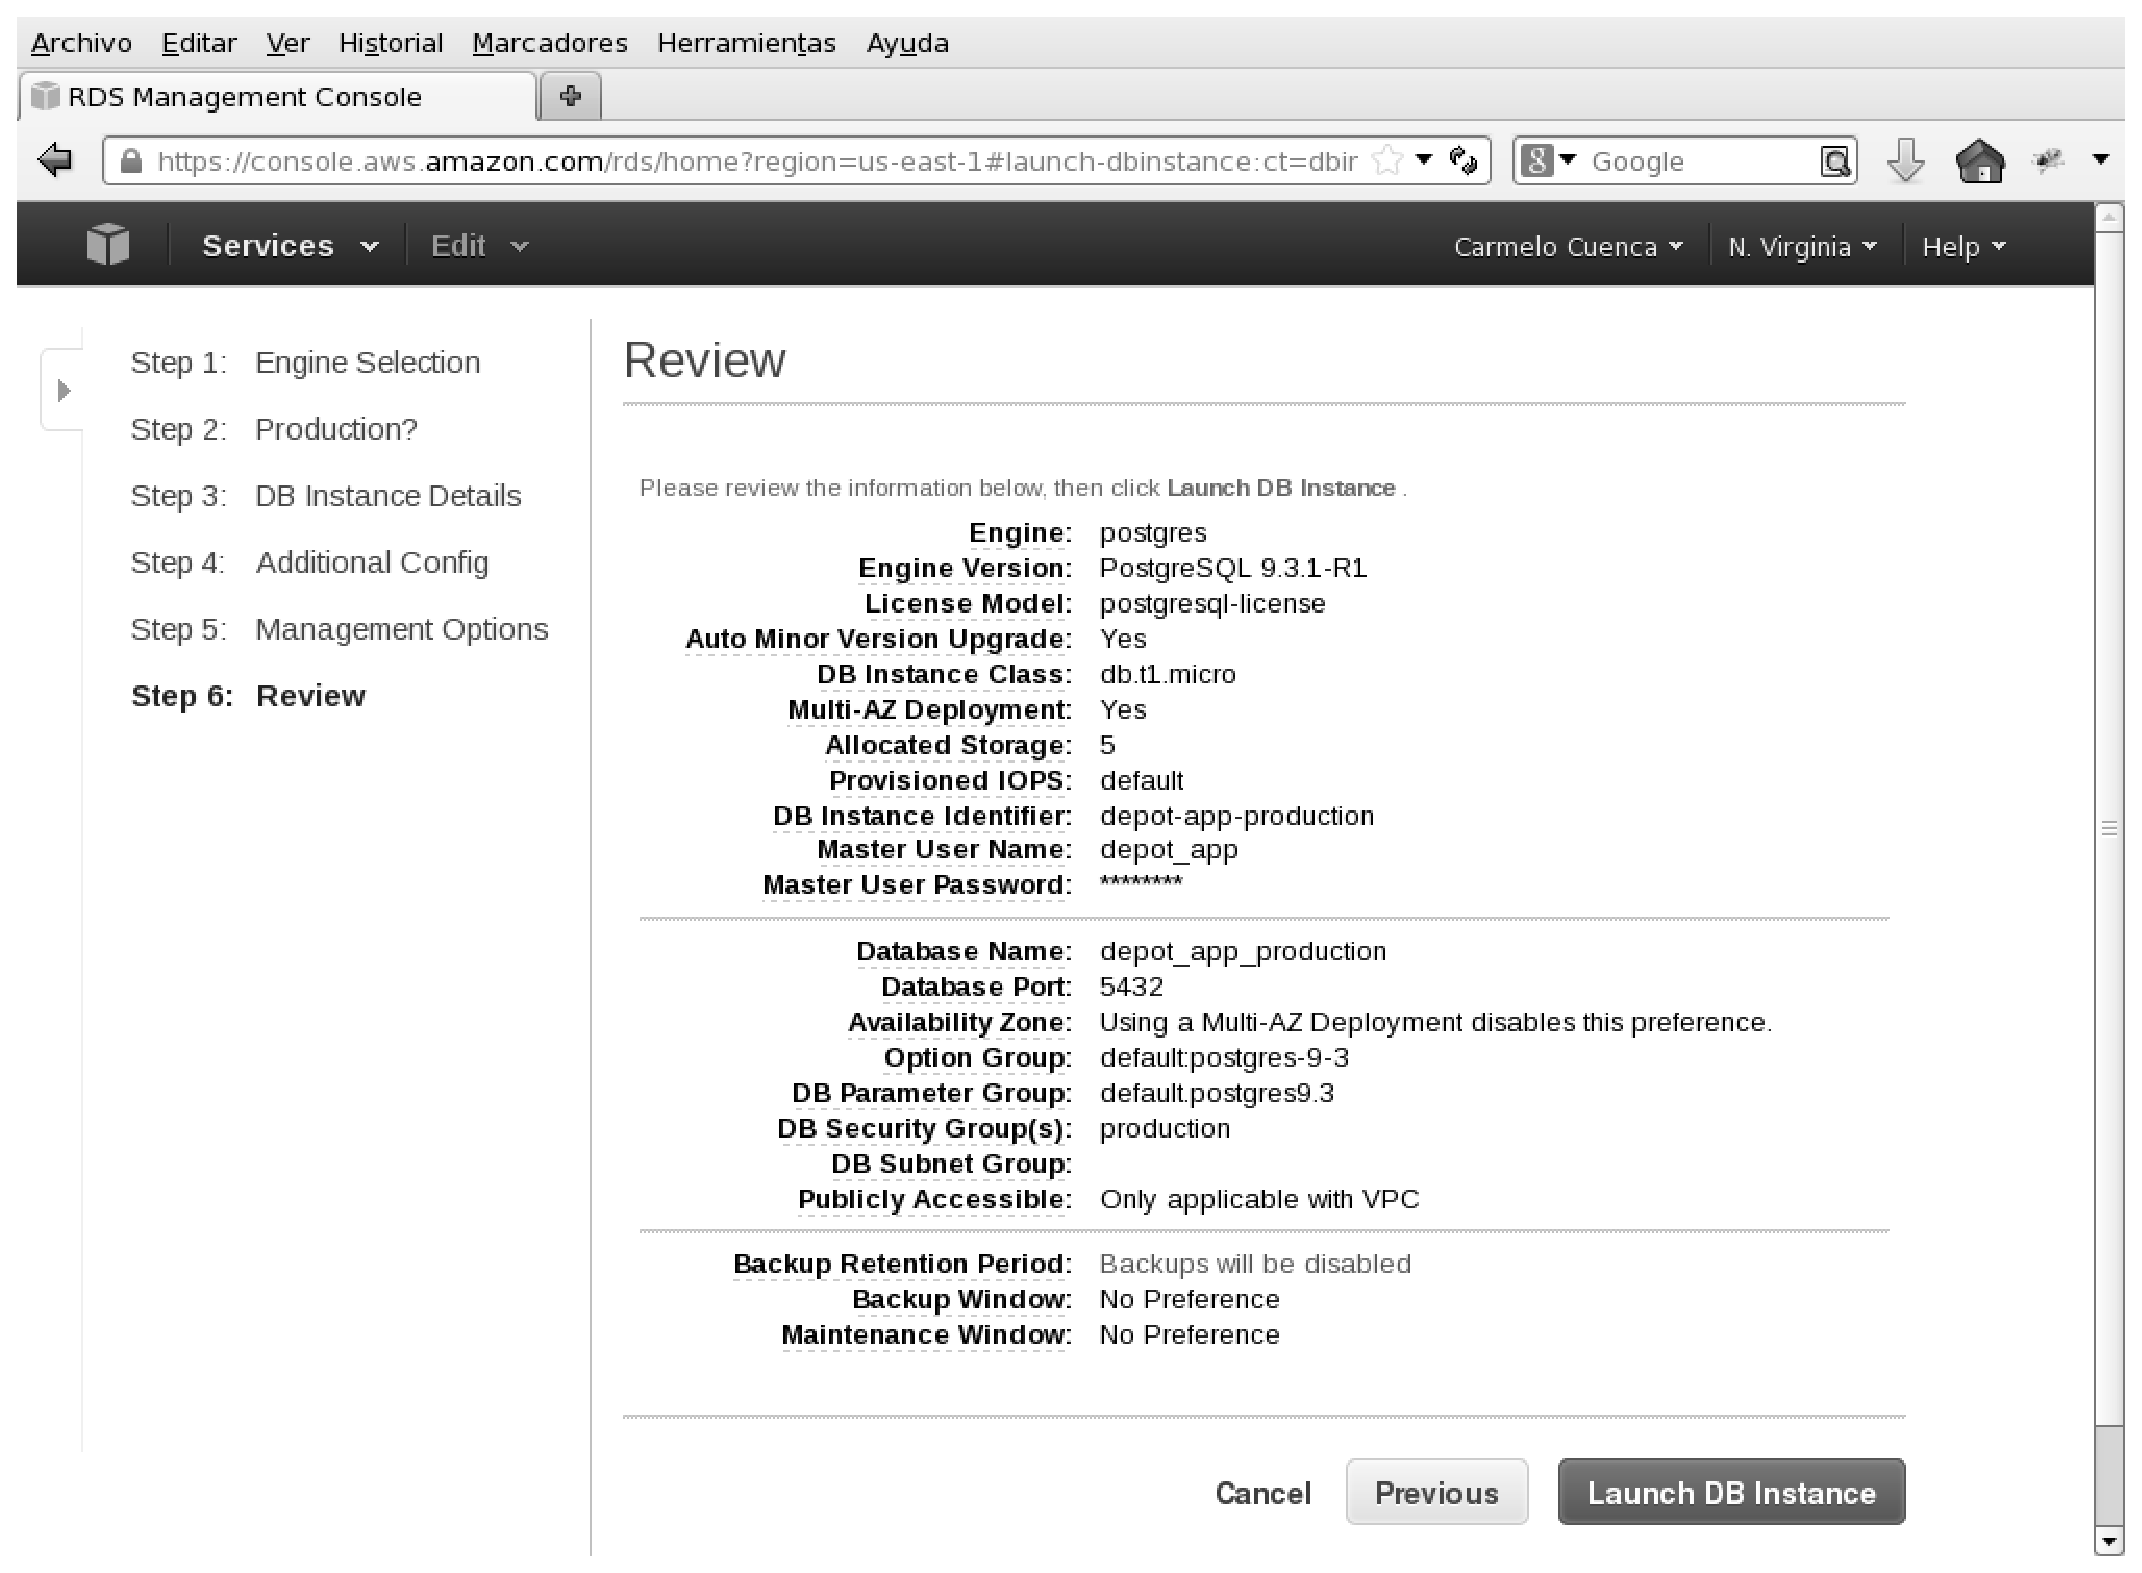
\includegraphics[scale=0.25]{rds.eps}
\end{center}
\end{frame}
%%%%%%%%%%%%%%%%%%%%%%%%%%%%%%%%%%%%%%%%%%%%%%%%%%%%%%%%%%%%%%%%%%%%%%%%%%%%%%
\begin{frame}[fragile, allowframebreaks]
\frametitle{DB Security Groups}
\begin{itemize}
\item Create a DB security group through the AWS Console and add the authorizations (as you did when you created your EC2 instances)
\item For now, we will allow everyone access to the DB instances in this group. Later, we’ll restrict that access again
\item Use port number \texttt{5432}
\end{itemize}

\end{frame}
%%%%%%%%%%%%%%%%%%%%%%%%%%%%%%%%%%%%%%%%%%%%%%%%%%%%%%%%%%%%%%%%%%%%%%%%%%%%%%
\begin{frame}[fragile, allowframebreaks]
\frametitle{Creating a RDS Instance}
\begin{itemize}
 \item Engine Selection (PostgreSQL)
 \item Production? Do you plan to use this database for production purposes?
    \begin{itemize}
      \item Multi-AZ Deployment for high availability (99.95\% monthly up time SLA). Provisioned IOPS Storage for fast, consistent performance
      \item Instance is intended for use outside of production or under the \alert{RDS Free Usage Tier}
    \end{itemize}
 \item DB Instance Details (Choose ``depot-app-production'' like \texttt{DB Instance Identifier} (hint: \texttt{DB Instance Identifier} must contain only letters, digits, or hyphens) and \texttt{Master Password} must be at least 8 characteres)
  \item Additional Config (Choose ``depot\_app\_production'' like \texttt{Database Name:} and ``production'' like \texttt{DB Security Group(s):})
  \item Management Options (Choose ``No'' for \texttt{Enabled Automatic Backups:}) 
  \item Review \& Launch DB Instance
  \end{itemize}
\end{frame}
%%%%%%%%%%%%%%%%%%%%%%%%%%%%%%%%%%%%%%%%%%%%%%%%%%%%%%%%%%%%%%%%%%%%%%%%%%%%%%%%%%%%%%%%%%%%%%%%%%%%%%%%%%%%%%%%%%%%%%%%%%%%%%%%%%%%%%%%%%
\begin{frame}[fragile, allowframebreaks]
\frametitle{Test a \acrshort{rds} Instance}
\begin{itemize}
 \item \texttt{pgsql} is a PostreSQL client. Test with it your \acrshort{rds} instance 
 \lstset{language=shell, breaklines=true}
  \begin{lstlisting}[escapechar=!]
  $ psql -W -h depot-app-production.ccoguny6ikux.us-east-1.rds.amazonaws.com  depot_app_production depot_app
  !\outputcommand{Contraseña para usuario depot\_app:\\
psql (9.3.2, servidor 9.3.1)\\
\dots}!
 \end{lstlisting}
\item Use \texttt{$\backslash q$} command to exit 
 \end{itemize}
\end{frame}
%%%%%%%%%%%%%%%%%%%%%%%%%%%%%%%%%%%%%%%%%%%%%%%%%%%%%%%%%%%%%%%%%%%%%%%%%%%%%%%%%%%%%%%%%%%%%%%%%%%%%%%%%%%%%%%%%%%%%%%%%%%%%%%%%%%%%%%%%%
\begin{frame}[fragile, allowframebreaks]
\frametitle{Cloud PostgreSQL Database in Production Environments}
\begin{itemize}
\item Start and login in the \acrshort{ec2} instance

\lstset{language=shell, escapechar=!}
\begin{lstlisting}
$ ssh -i your_key_file.pem root@ec2-nnn-nnn-nn-nnn.compute-1.amazonaws.com
# su -  depot_app
\end{lstlisting}

\item Edit \texttt{config/database.yml} file (configuration database file) in order to run the application with \texttt{PostgreSQL} \acrshort{rds}

\lstset{language=Ruby, style=eclipse, numbers=left}
\begin{lstlisting}[escapechar=!]
!\vdots!
production:
  adapter: postgresql
  encoding: unicode
  database: depot_app_production
  pool: 5
#!\circled{1}!
  host: depot-app-production.ccoguny6ikux.us-east-1.rds.amazonaws.com
  port: 5432
  username: depot_app
  password: 12345678
!\vdots!
\end{lstlisting}

\item Stop the PostgreSQL daemon

\lstset{language=shell, escapechar=!}
\begin{lstlisting}[escapechar=!]
# /etc/init.d/postgresql-9.3 stop
# chkconfig postgresql-9.3 off
# chkconfig --list postgresql-9.3
\end{lstlisting}

\item Migrate \texttt{depot\_app\_production} tables and  seed the data

\lstset{language=shell}
\begin{lstlisting}[numbers=none, escapechar=!]
$ rake db:migrate RAILS_ENV=production
$ rake db:seed RAILS_ENV=production
\end{lstlisting}

\item Restart unicorn server
\lstset{language=shell, escapechar=!}
\begin{lstlisting}[escapechar=!]
# /etc/init.d/unicorn_depot_app restart
\end{lstlisting}

\item Curl your application and \dots 

\begin{lstlisting}[escapechar=!]
$ curl http://my.public.dns.amazonaws.com:5000
\end{lstlisting} 

 \end{itemize}
\end{frame}

%%%%%%%%%%%%%%%%%%%%%%%%%%%%%%%%%%%%%%%%%%%%%%%%%%%%%%%%%%%%%%%%%%%%%%%%%%%%%%%%%%%%%%%%%%%%%%%%%%%%%%%%%%%%%%%%%%%%%%%%%%%%%%%%%%%%%%%%%%
\comment{
\section{Web Server Benchmarking}
\begin{frame}[fragile]
\frametitle{Web Server Benchmarking}
\begin{itemize}
  \item Web Sites \url{WebPageTest.org}
  \item Apache  \texttt{JMeter}
  \item Tools \texttt{httperf}, \texttt{ab} (Apache Bench)
\lstset{language=shell}
\begin{lstlisting}[escapechar=!]
$ ab -n request -c concurrency [http[s]://]hostname[:port]/path
\end{lstlisting}
   \end{itemize}
\end{frame}
%%%%%%%%%%%%%%%%%%%%%%%%%%%%%%%%%%%%%%%%%%%%%%%%%%%%%%%%%%%%%%%%%%%%%%%%%%%%%%%%%%%%%%%%%%%%%%%%%%%%%%%%%%%%%%%%%%%%%%%%%%%%%%%%%%%%%%%%%%

%%%%%%%%%%%%%%%%%%%%%%%%%%%%%%%%%%%%%%%%%%%%%%%%%%%%%%%%%%%%%%%%%%%%%%%%%%%%%%%%%%%%%%%%%%%%%%%%%%%%%%%%%%%%%%%%%%%%%%%%%%%%%%%%%%%%%%%%%%

\begin{frame}[fragile, allowframebreaks]
\frametitle{Testing a Web Application}
\begin{itemize}
\item Tail user the Apachelog files  as \texttt{root}  in \acrshort{ec2} in order to check Apache Server
\lstset{language=shell}
\begin{lstlisting}[escapechar=!]
# tail -f /var/log/httpd/depot_app*
\end{lstlisting}
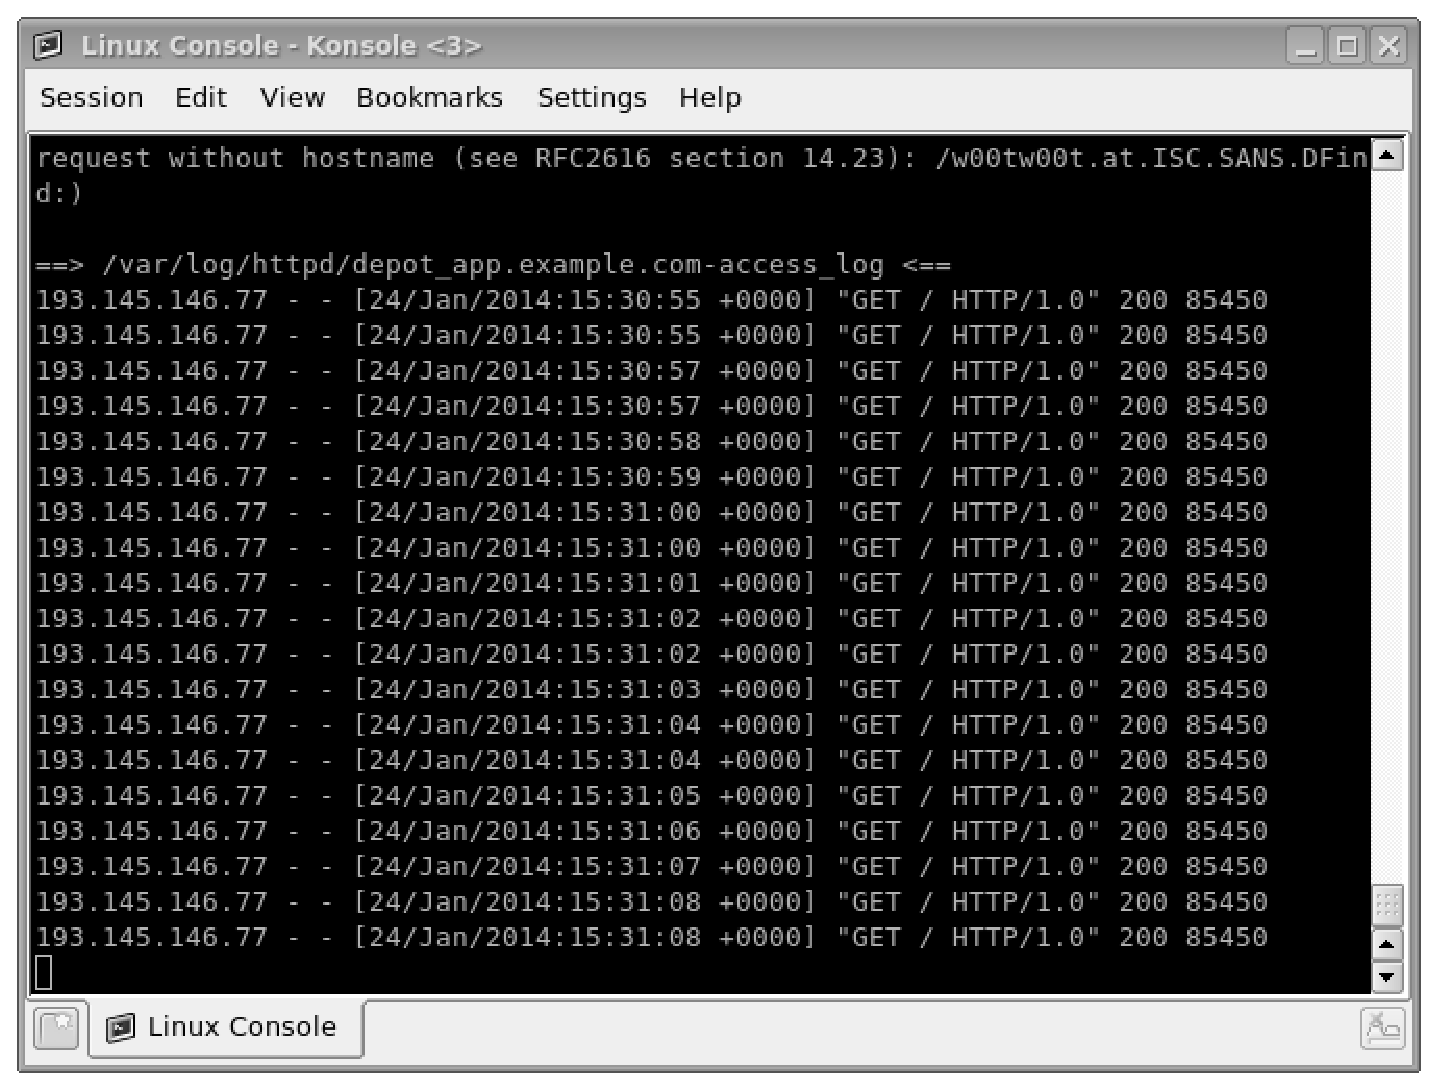
\includegraphics[scale=0.15]{logapache.eps}

\item Tail the Unicorn log files as \texttt{depot\_app} in \acrshort{ec2} in order to check Unicorn Server
\lstset{language=shell}
\begin{lstlisting}[escapechar=!]
$ tail -f log/production.log log/unicorn.std*
\end{lstlisting}
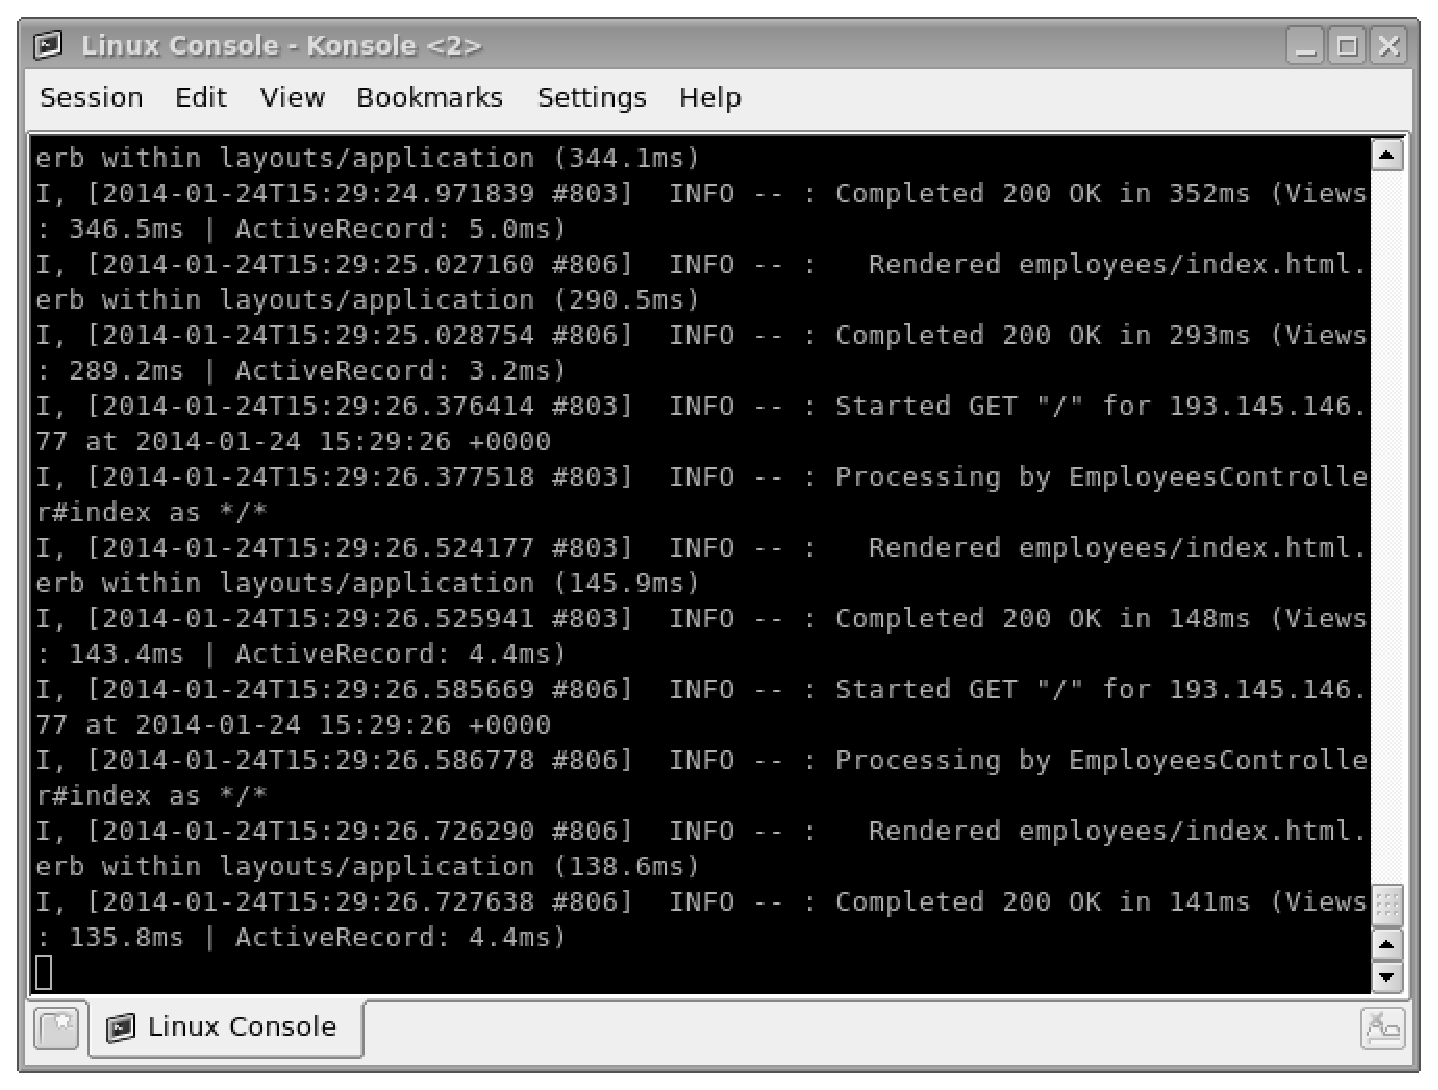
\includegraphics[scale=0.15]{lograils.eps}

\item Run JMeter (More info in \url{http://jmeter.apache.org/index.html}) and create a test plan
\begin{center}
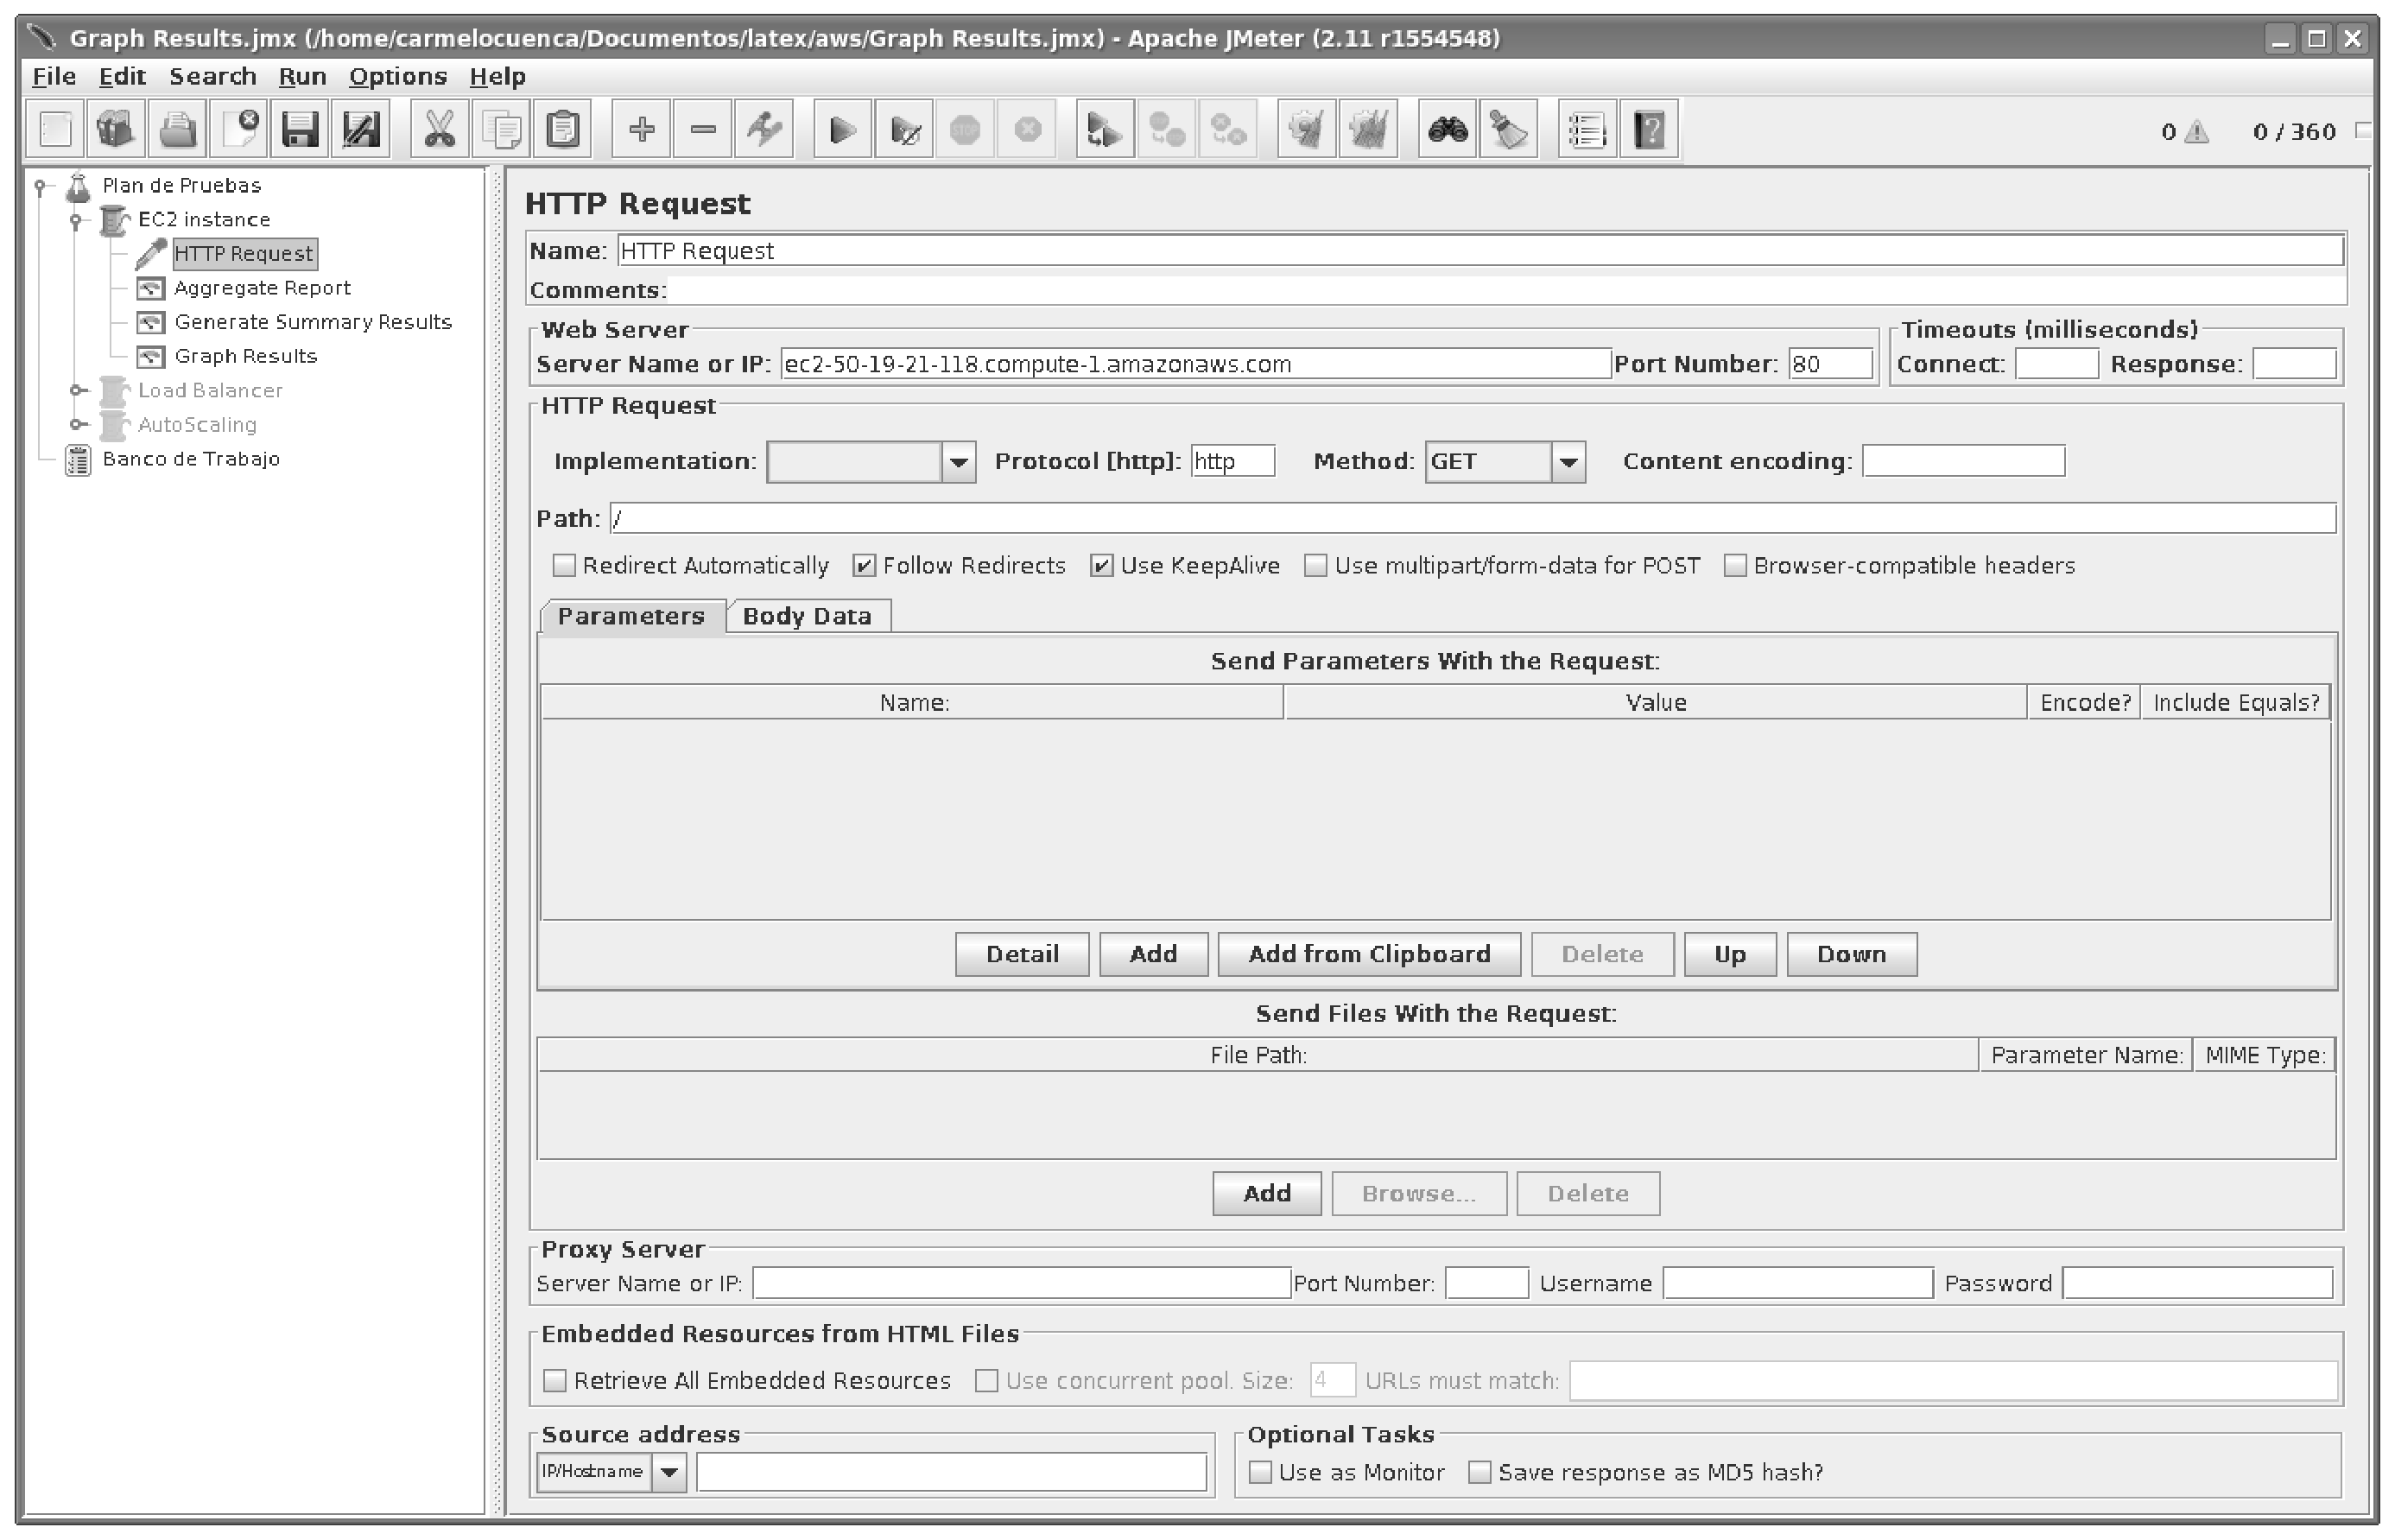
\includegraphics[scale=0.15]{plandeprueba.eps}
\end{center}
\begin{center}
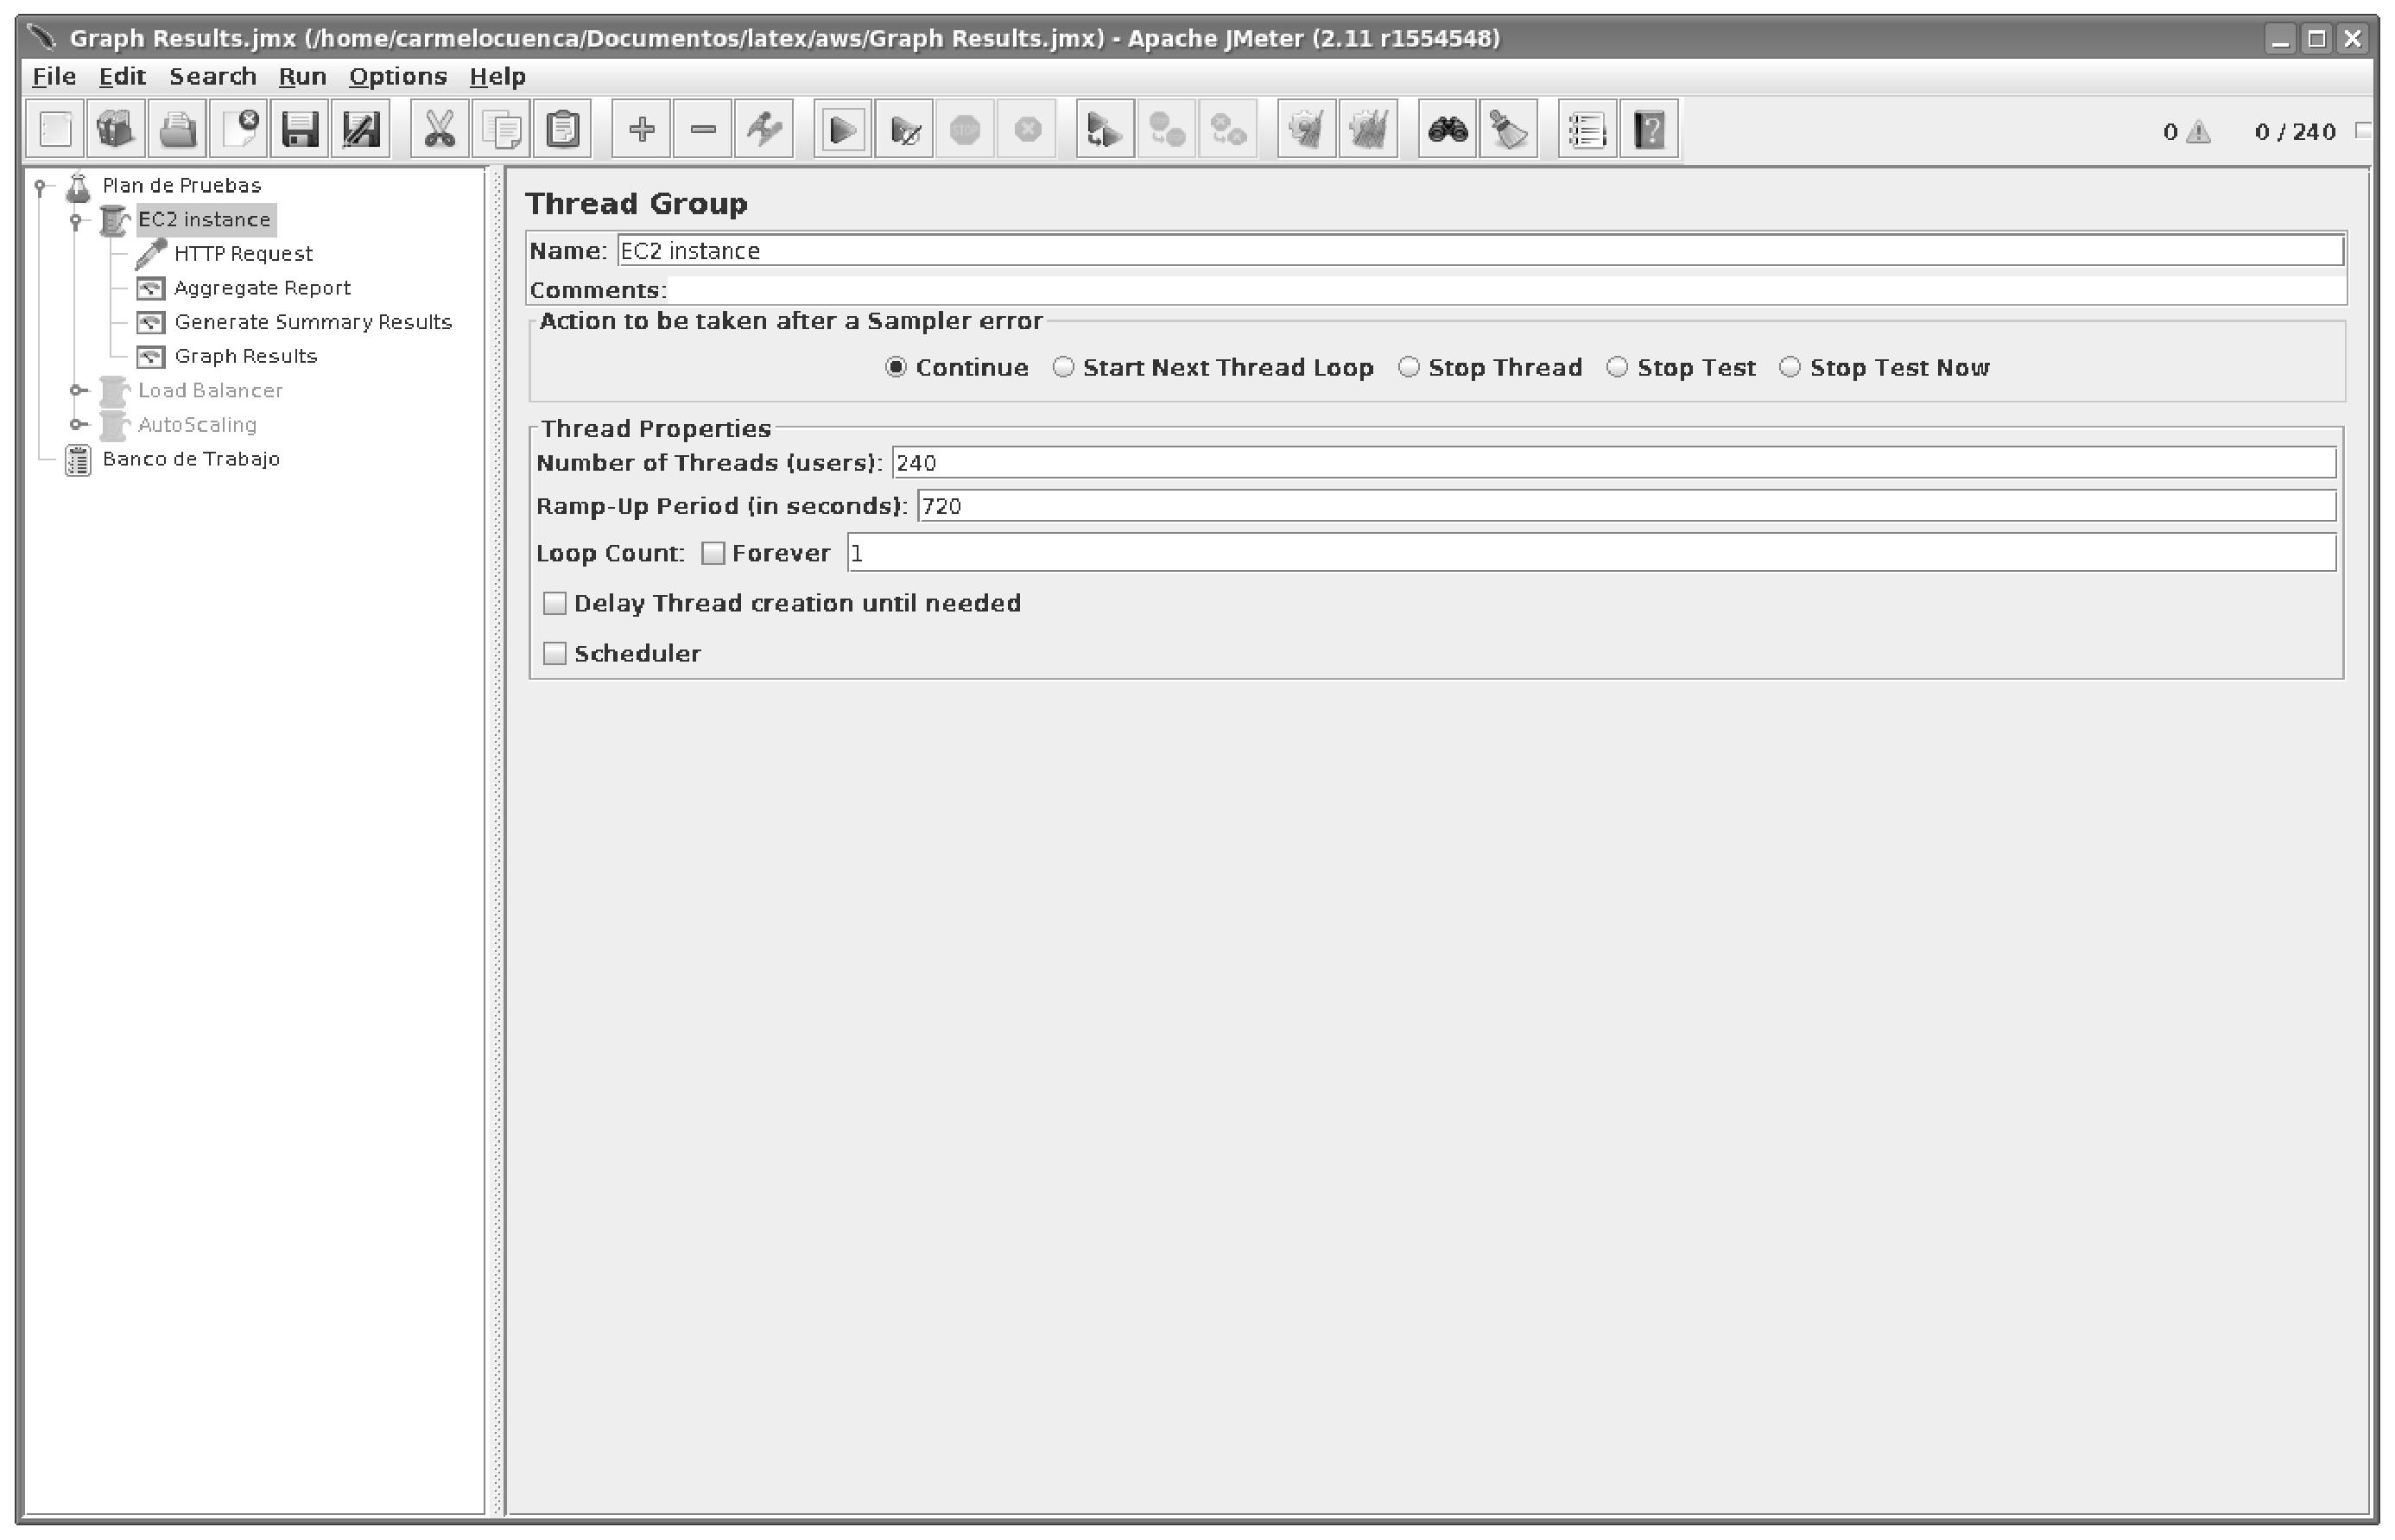
\includegraphics[scale=0.15]{plandeprueba1.eps}
\end{center}

\begin{enumerate}
\item Right-click on the Test Plan node and choose \texttt{Add - Threads (Users) - Thread Group}
\item Configure the thread group with 240 threads, a ramp-up period of 720 seconds (12 minutes), and a loop count of 1
\item Right-click on the new Thread Group node and choose \texttt{Add - Sampler - HTTP Request}
\item Enter your server host name or IP address ( omit the \texttt{http://} protocol prefix) and port (80 should be fine)
\item Enter \texttt{``/''} for the path to retrieve the home page from the site
\item Right-click on the Test Pl an node once again. Add the following listener nodes: \texttt{Generate Summary Results, Aggregate Report, and Graph Results}

\end{enumerate}

\item Monitoring results and CloudWatch metrics in the ``Monitoring Tab''
\begin{center}
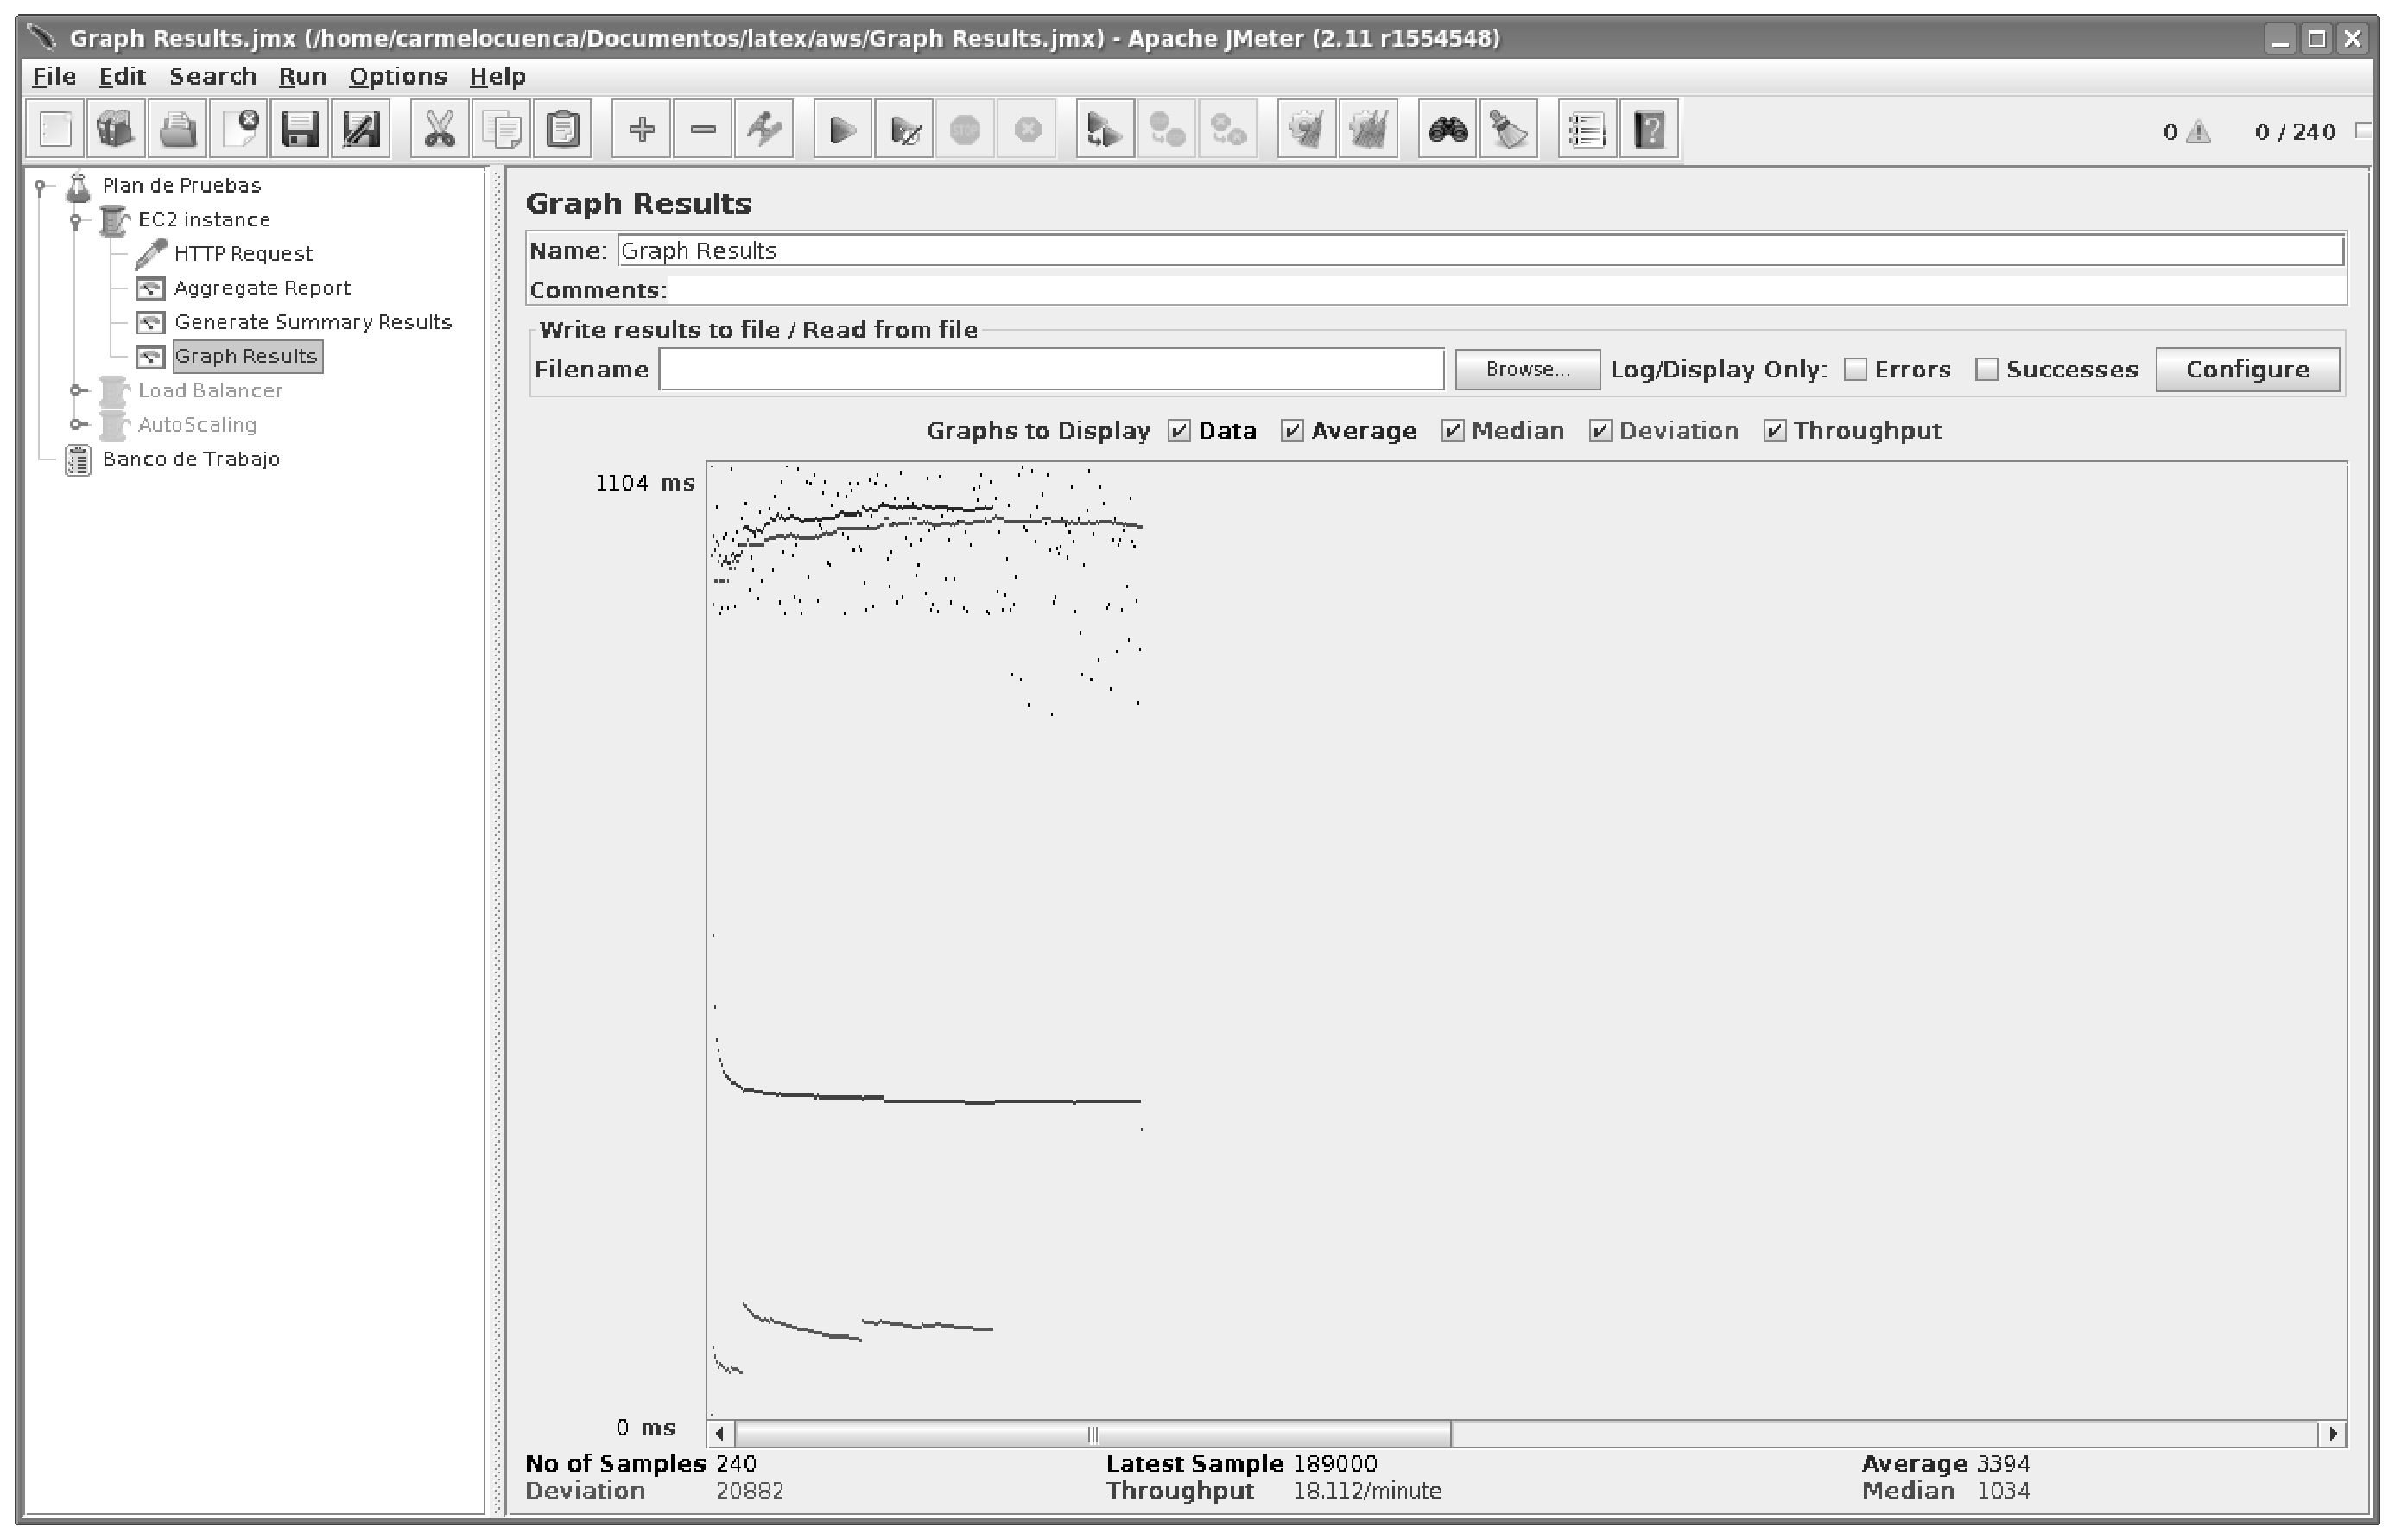
\includegraphics[scale=0.15]{plandeprueba2.eps}
\end{center}
\begin{center}
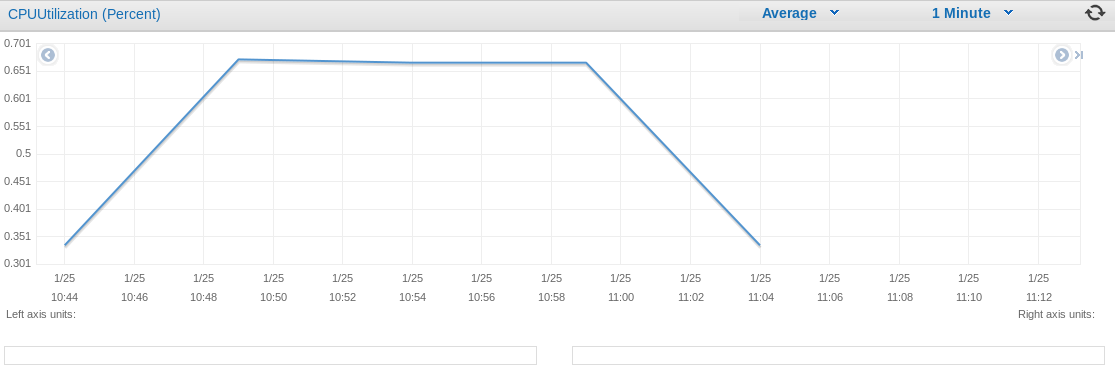
\includegraphics[scale=0.15]{cpuutilization.png}
\end{center}
\end{itemize}

\end{frame}
}
%%%%%%%%%%%%%%%%%%%%%%%%%%%%%%%%%%%%%%%%%%%%%%%%%%%%%%%%%%%%%%%%%%%%%%%%%%%%%%


\section{Amazon Machine Image (AMI)}
\begin{frame}[fragile, allowframebreaks]
\frametitle{Amazon Machine Image (AMI)}
\begin{enumerate}
\item You can customize the instance that you launch from a public \acrshort{ami} and then save that configuration as a custom \acrshort{ami} for your own use
\item Instances that you launch from your \acrshort{ami} use all the customizations that you've made
\end{enumerate}

\end{frame}
%%%%%%%%%%%%%%%%%%%%%%%%%%%%%%%%%%%%%%%%%%%%%%%%%%%%%%%%%%%%%%%%%%%%%%%%%%%%%%
%%%%%%%%%%%%%%%%%%%%%%%%%%%%%%%%%%%%%%%%%%%%%%%%%%%%%%%%%%%%%%%%%%%%%%%%%%%%%%
\begin{frame}[fragile, allowframebreaks]
\frametitle{Creating Your Own \acrshort{ami}}
\begin{enumerate}
\item In order to distinguish between \acrshort{ec2} machines we have written in the application layout (as user \texttt{depot\_app} )

\lstset{language=html, style=eclipse}
\begin{lstlisting}[escapechar=!]
# ~/public_html/depot_app/app/views/layouts/application.html.erb
!\vdots!
  <div id="main">
    <%= yield %>
    <%= Socket.ip_address_list.to_s %> # !\circled{1}!
  </div>
</div>
\end{lstlisting}

\item Create an \acrshort{ami} of our \acrshort{ec2} instance and launch a new clone of our \acrshort{ec2} machine
\begin{center}
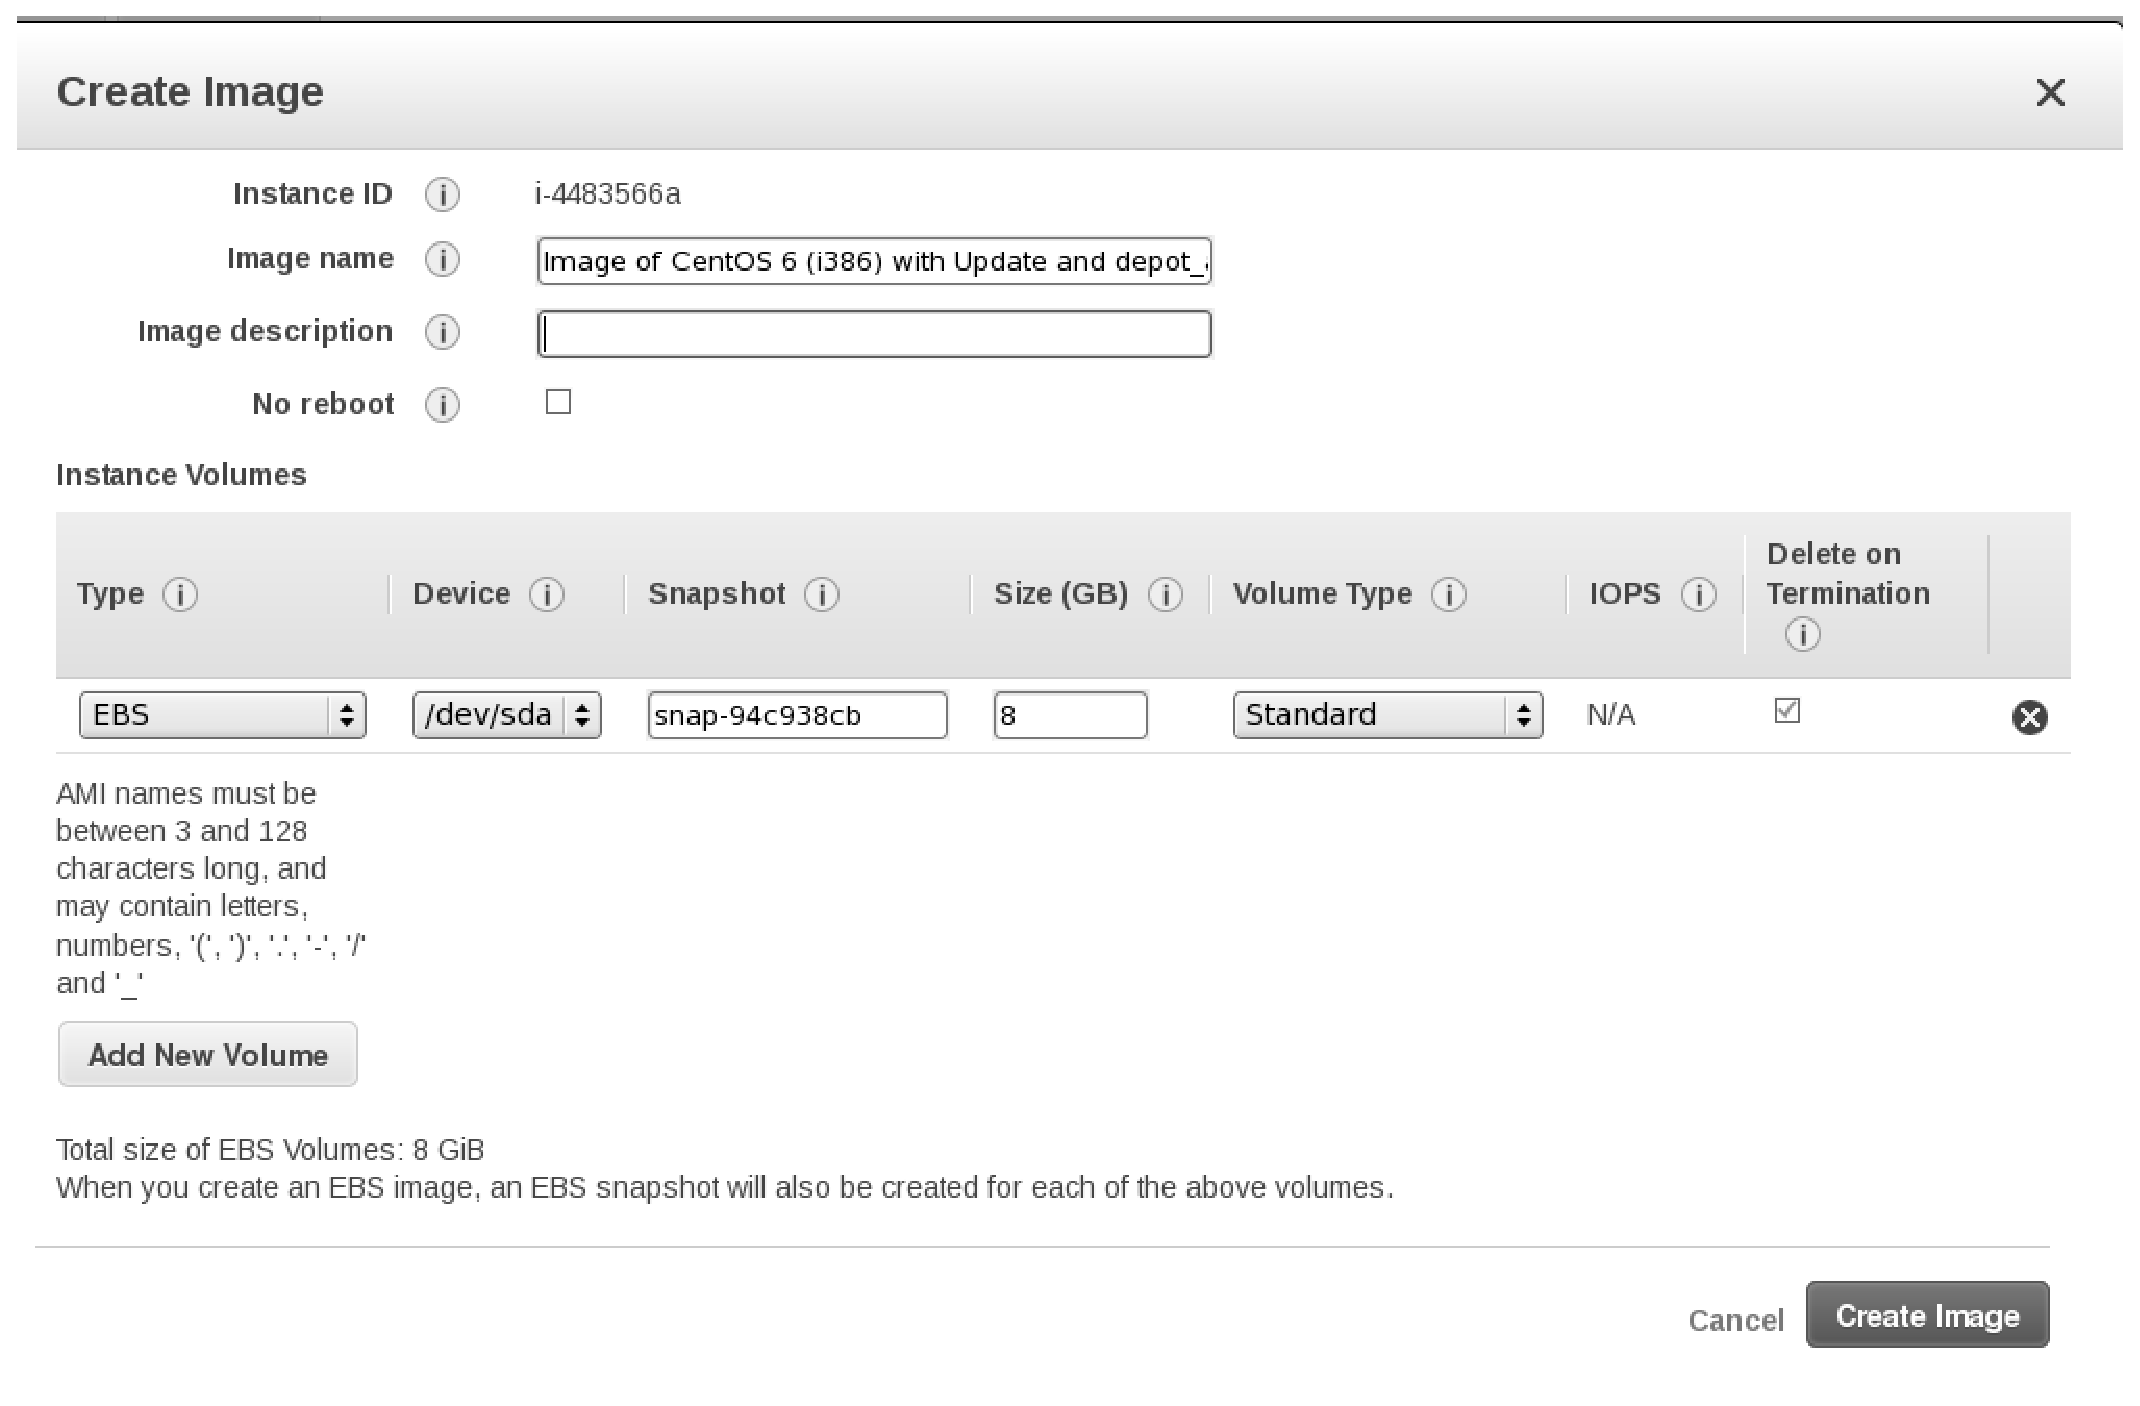
\includegraphics[scale=0.20]{createimage.eps}
\end{center}
\item Curl both IPs in order to test both \acrshort{ec2} instances
\end{enumerate}

\end{frame}
%%%%%%%%%%%%%%%%%%%%%%%%%%%%%%%%%%%%%%%%%%%%%%%%%%%%%%%%%%%%%%%%%%%%%%%%%%%%%%
%%%%%%%%%%%%%%%%%%%%%%%%%%%%%%%%%%%%%%%%%%%%%%%%%%%%%%%%%%%%%%%%%%%%%%%%%%%%%%
\section{Elastic Load Balancing}
%%%%%%%%%%%%%%%%%%%%%%%%%%%%%%%%%%%%%%%%%%%%%%%%%%%%%%%%%%%%%%%%%%%%%%%%%%%%%%
\begin{frame}[fragile, allowframebreaks]
\frametitle{Elastic Load Balancing}
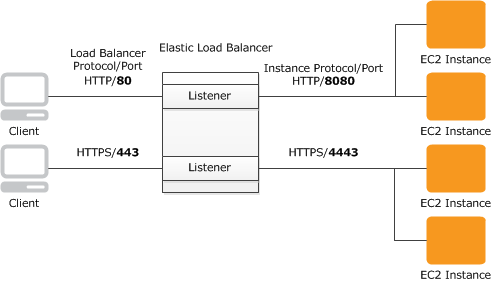
\includegraphics[width=0.75 \textwidth]{elb-listeners.png}
\begin{itemize}
\item Load balancing is ``a technique to distribute workload evenly across
two or more computers, network links, CPUs, hard drives, or other resources, in order
to get optimal resource utilization, maximize throughput, minimize response time, and
avoid overload.'' (Wikipedia)
\item  \acrfull{elb} checks the health of the
instances and will not route traffic to unhealthy instances
\item \acrshort{elb} is not a dedicated program or a hardware device; it is a load-balancing service. As
a service, it can automatically scale its capacity depending on incoming traffic. As a
result, an \acrshort{elb} is not referenced by an IP address, but by a fully qualified domain name
\end{itemize}
\end{frame}
%%%%%%%%%%%%%%%%%%%%%%%%%%%%%%%%%%%%%%%%%%%%%%%%%%%%%%%%%%%%%%%%%%%%%%%%%%%%%%
\begin{frame}[fragile, allowframebreaks]
\frametitle{Creating a ELB}
\begin{enumerate}	
\item Summary
\begin{center}
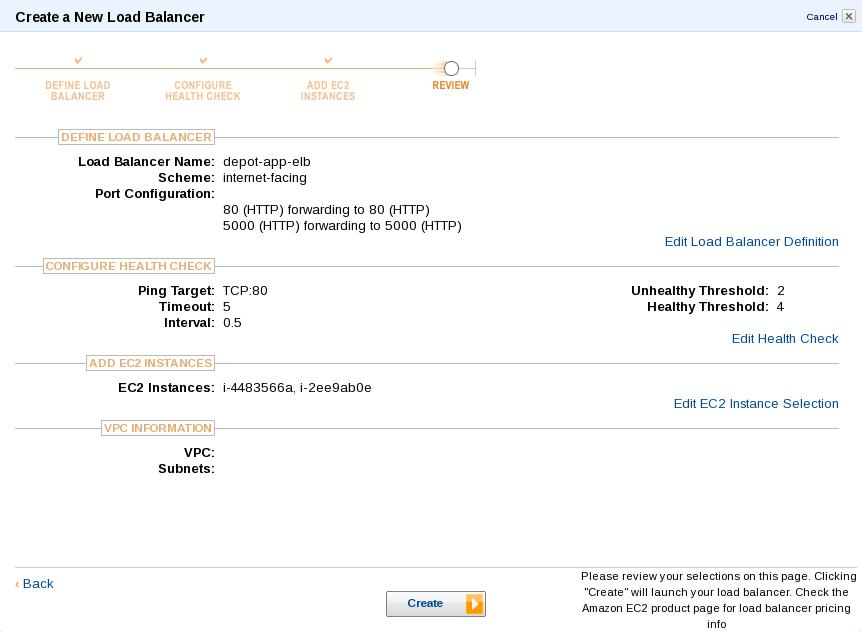
\includegraphics[scale=0.2]{createelb3.jpg}
\end{center}
\item Define Load Balancer
\begin{center}
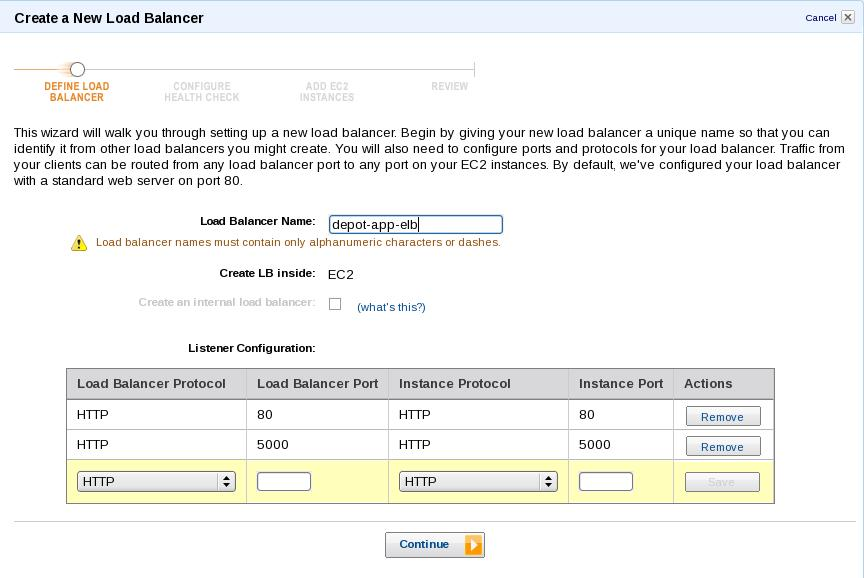
\includegraphics[scale=0.2]{define-load-balancer.jpg}
\end{center}	
\item Configure Health Check (\alert{Use protocol TCP and set \texttt{Healthy Threshold:} to 4})
\begin{center}
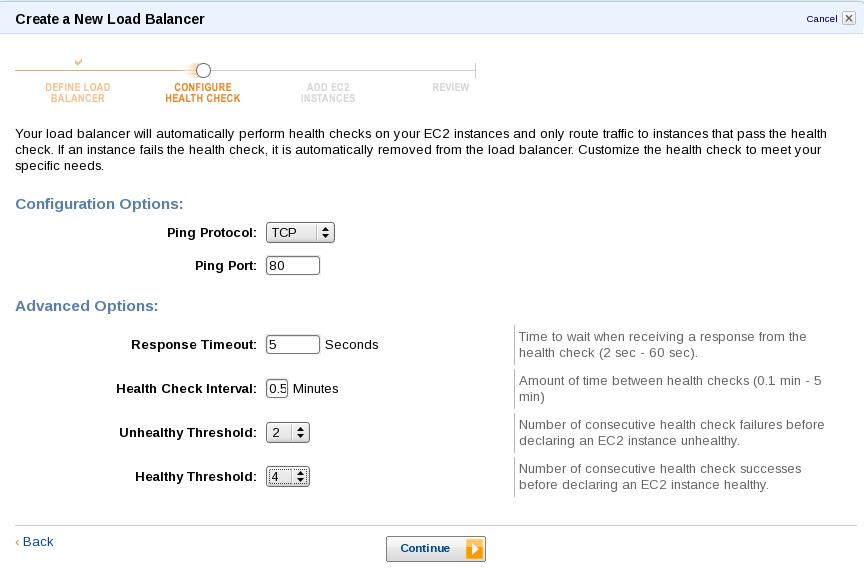
\includegraphics[scale=0.2]{createelb1.jpg}
\end{center}
\item Add \acrshort{ec2} instances (\alert{Instances should be launched in the same zone})
\begin{center}
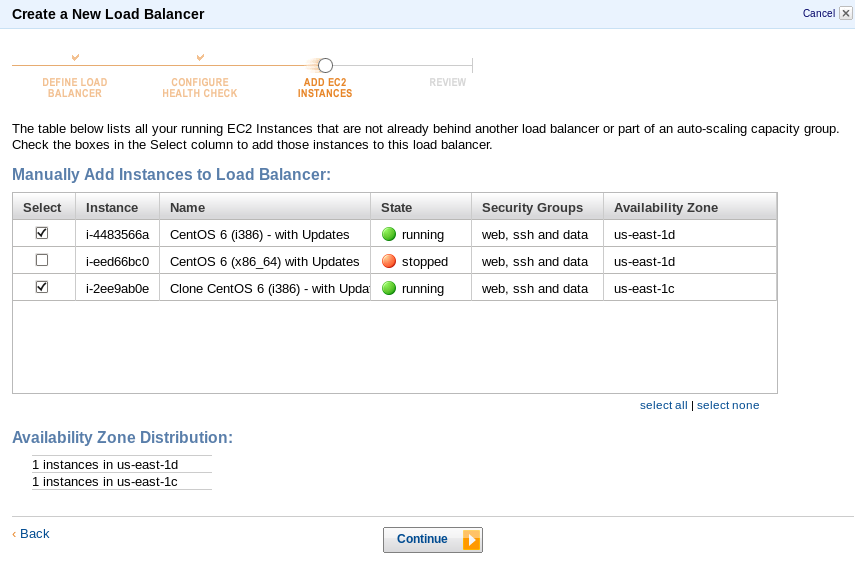
\includegraphics[scale=0.25]{createaelb1.png}
\end{center}	
\item Review
\end{enumerate}

\end{frame}
%%%%%%%%%%%%%%%%%%%%%%%%%%%%%%%%%%%%%%%%%%%%%%%%%%%%%%%%%%%%%%%%%%%%%%%%%%%%%%
%%%%%%%%%%%%%%%%%%%%%%%%%%%%%%%%%%%%%%%%%%%%%%%%%%%%%%%%%%%%%%%%%%%%%%%%%%%%%%
\begin{frame}[fragile]
\frametitle{Testing a ELB}
\
\begin{itemize}	
\item Curl the fully qualified domain name of \acrshort{elb} in order to check the \acrshort{elb} 
\lstset{language=shell}
\begin{lstlisting}[escapechar=!]
$ curl http://depot-app-1557778043.us-east-1.elb.amazonaws.com: 2>/dev/null | grep 'Addrinfo:' | gawk '{print $4}'
!\outputcommand{10.192.182.72\&gt;,}!
$ curl http://depot-app-1557778043.us-east-1.elb.amazonaws.com: 2>/dev/null | grep 'Addrinfo:' | gawk '{print $4}'
!\outputcommand{10.210.202.71\&gt;,}!
\end{lstlisting}
\end{itemize}

\end{frame}
%%%%%%%%%%%%%%%%%%%%%%%%%%%%%%%%%%%%%%%%%%%%%%%%%%%%%%%%%%%%%%%%%%%%%%%%%%%%%%
%%%%%%%%%%%%%%%%%%%%%%%%%%%%%%%%%%%%%%%%%%%%%%%%%%%%%%%%%%%%%%%%%%%%%%%%%%%%%%
\section{AutoScaling}
%%%%%%%%%%%%%%%%%%%%%%%%%%%%%%%%%%%%%%%%%%%%%%%%%%%%%%%%%%%%%%%%%%%%%%%%%%%%%%
%%%%%%%%%%%%%%%%%%%%%%%%%%%%%%%%%%%%%%%%%%%%%%%%%%%%%%%%%%%%%%%%%%%%%%%%%%%%%%%%%%%%%%%%%%%%%%%%%%%%%%%%%%%%%%%%%%%%%%%%%%%%%%%%%%%%%%%%%%
\begin{frame}[fragile, allowframebreaks]
\frametitle{Auto Scaling}
\begin{itemize}
 \item Auto Scaling is a web service that enables you to automatically launch or terminate \acrshort{ec2} instances based on user-defined policies, health status checks, and schedules
 \item Scaling is the ability to increase or decrease the compute capacity of your application by either changing the number of servers (horizontal scaling) or changing the size of the servers (vertical scaling)
\item The decision when to scale vertically and when to scale horizontally depends on factors such as your use case, cost, performance, and infrastructure
\item Auto Scaling allows you to scale your compute resources dynamically and predictably:
\begin{itemize}
 \item Dynamically based on conditions specified by you (for example, increasing CPU utilization of your \acrshort{ec2} instance)
 \item Predictably according to a schedule defined by you (for example, every Friday at 13:00:00)
\end{itemize}



\pagebreak

\item You need to configure your autoscaling:

\begin{columns}
\column{0.7 \textwidth}
\begin{enumerate}
\item Create a launch configuration. First, define a template that your Auto Scaling group will use to launch instances
\item Create a autoscaling group. Your group will maintain this number of instances, and replace any that become unhealthy or impaired.
You can optionally configure your group to adjust in capacity according to demand, in response to Amazon CloudWatch metrics
\end{enumerate}
\column{0.3 \textwidth}
\begin{center}
 \item 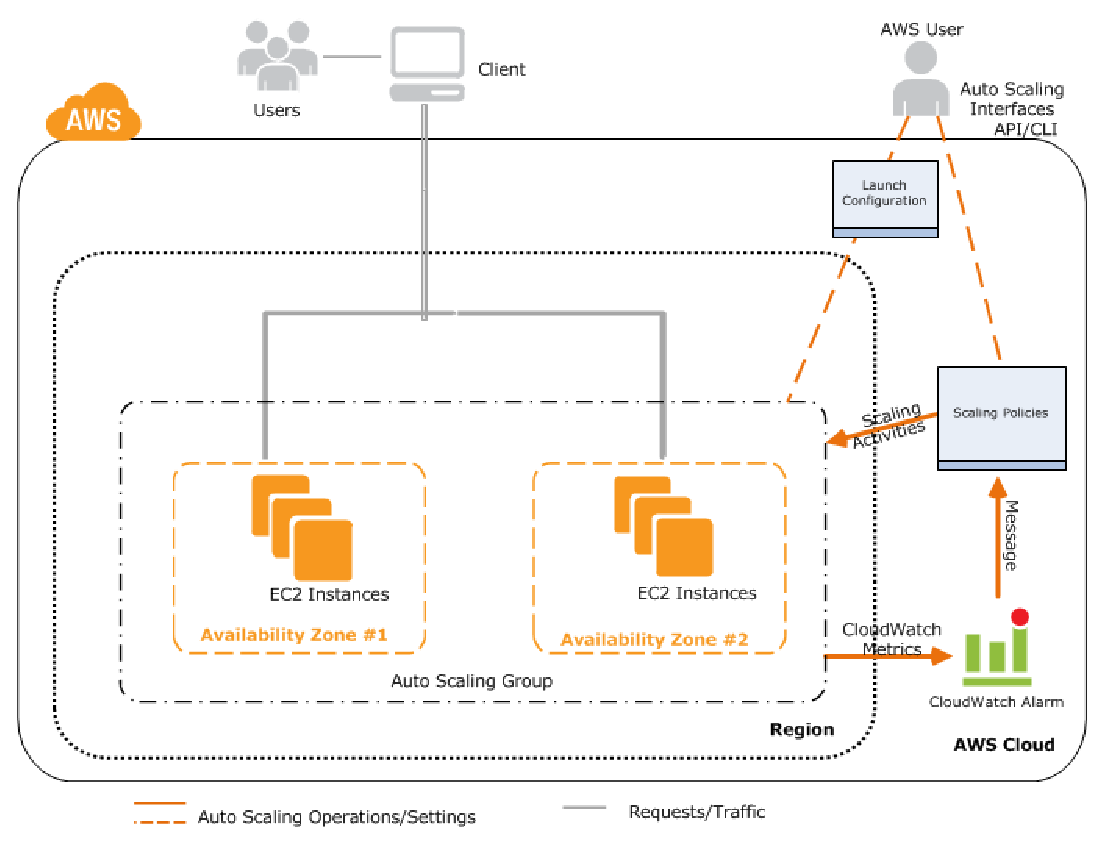
\includegraphics[scale=0.2]{AS-WorkFlow.eps}
\end{center}
\end{columns}

\end{itemize}
\end{frame}

%%%%%%%%%%%%%%%%%%%%%%%%%%%%%%%%%%%%%%%%%%%%%%%%%%%%%%%%%%%%%%%%%%%%%%%%%%%%%%%%%%%%%%%%%%%%%%%%%%%%%%%%%%%%%%%%%%%%%%%%%%%%%%%%%%%%%%%%%%
\begin{frame}[fragile]
\frametitle{Launch Configuration}
\begin{enumerate}
\item Choose \acrshort{ami} (\texttt{Clone Centos (i386) - with Updates - ami-af330fc6})
\item Choose Instance Type \texttt{t1.micro}
\item Configure details \texttt{Name: `depot-app-launch-configuration', Monitoring: `Yes'}
\item Add Storage
\item Configure Security Group \texttt{Name: `web, ssh and data', Description: `Allow http, https, ssh, 3000, 5000'}
\item Review
\end{enumerate}
\end{frame}
%%%%%%%%%%%%%%%%%%%%%%%%%%%%%%%%%%%%%%%%%%%%%%%%%%%%%%%%%%%%%%%%%%%%%%%%%%%%%%%%%%%%%%%%%%%%%%%%%%%%%%%%%%%%%%%%%%%%%%%%%%%%%%%%%%%%%%%%%%

\begin{frame}[fragile, allowframebreaks]
\frametitle{Auto Scaling Group}
\begin{center}
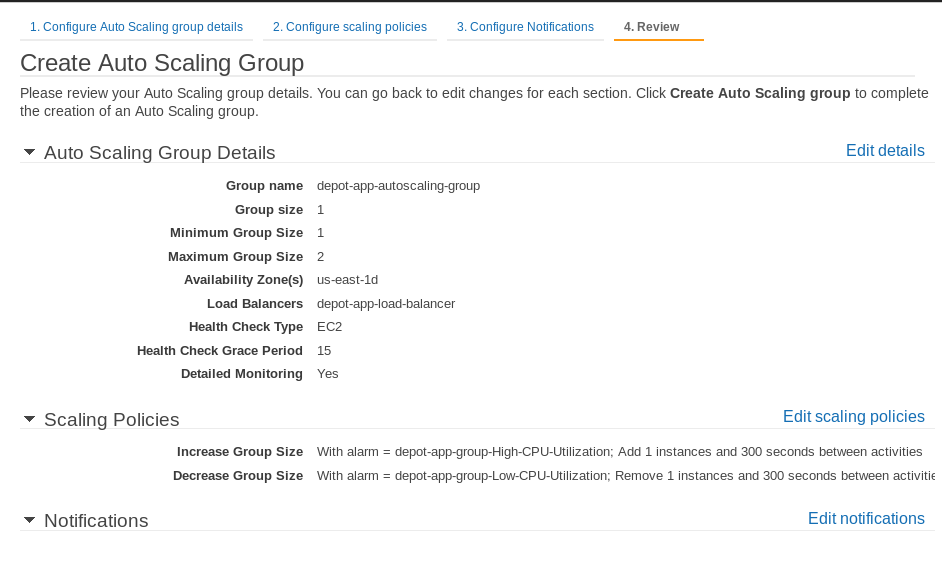
\includegraphics[scale=0.30]{review-autoscale.png}
\end{center}
\begin{enumerate}
\item Configure Auto Scaling group details'\\
\alert{Don't forget to tick ``Receive traffic from Elastic Load Balancer'' and set it properly}\\
\alert{Don't forget to choose an instace zone}
\begin{center}
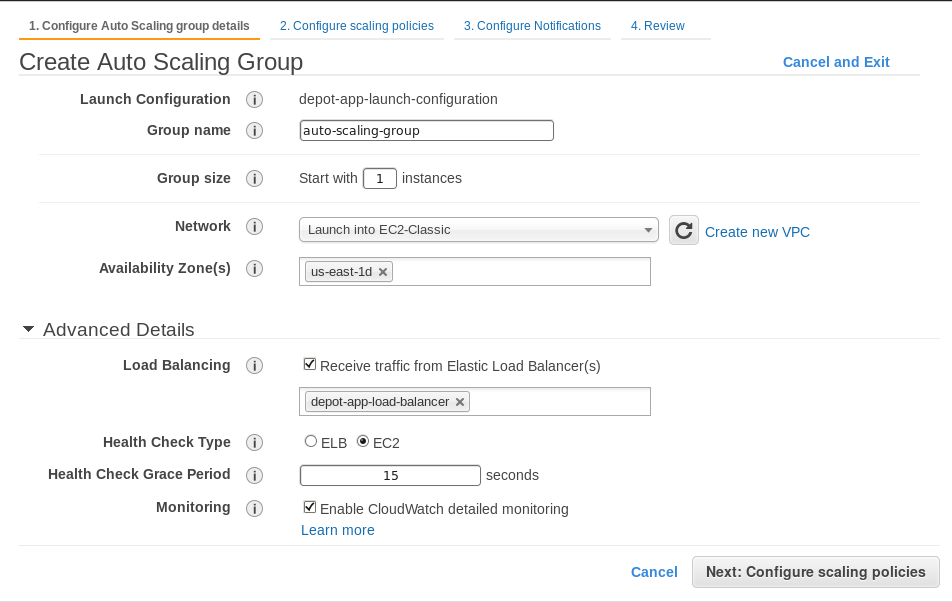
\includegraphics[scale=0.20]{create-auto-scaling01.png}
\end{center}
\item Configure scaling policies. Define two alarms: \texttt{CPUUtilization >= 50 for 60 seconds} and \texttt{CPUUtilization <= 25 for 60 seconds}
\begin{center}
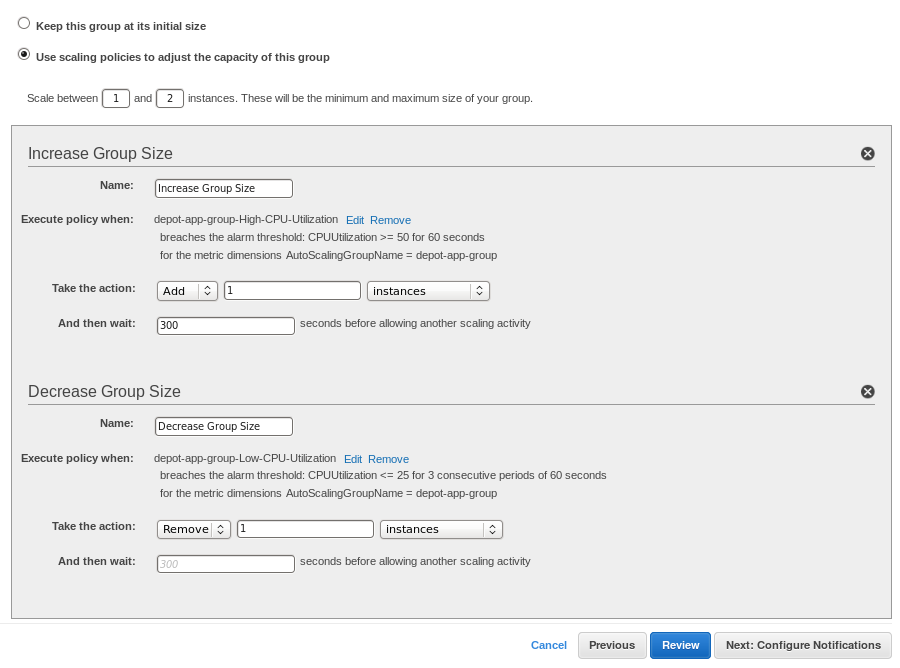
\includegraphics[scale=0.25]{configure-scaling-policies.png}
\end{center}
\item Configure Notifications (successful launch of an instance, failed instance launch, instance termination, failed instance termination \dots)
\item Review
\end{enumerate}

\end{frame}
%%%%%%%%%%%%%%%%%%%%%%%%%%%%%%%%%%%%%%%%%%%%%%%%%%%%%%%%%%%%%%%%%%%%%%%%%%%%%%%%%%%%%%%%%%%%%%%%%%%%%%%%%%%%%%%%%%%%%%%%%%%%%%%%%%%%%%%%%%
%%%%%%%%%%%%%%%%%%%%%%%%%%%%%%%%%%%%%%%%%%%%%%%%%%%%%%%%%%%%%%%%%%%%%%%%%%%%%%%%%%%%%%%%%%%%%%%%%%%%%%%%%%%%%%%%%%%%%%%%%%%%%%%%%%%%%%%%%%
\begin{frame}[fragile]
\frametitle{Testing the AutoScaling Group}

\lstset{language=shell}
\begin{itemize}
 \item We have to define a web load and check that the AutoScaling Group work properly
\begin{center}
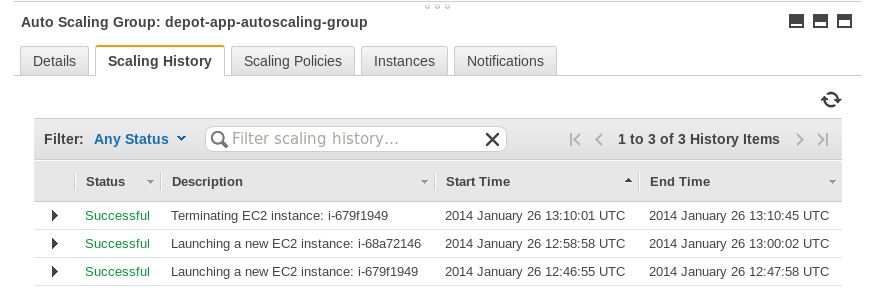
\includegraphics[scale=0.45]{autoscalingwork.png}
\end{center}
\end{itemize}

\end{frame}
%%%%%%%%%%%%%%%%%%%%%%%%%%%%%%%%%%%%%%%%%%%%%%%%%%%%%%%%%%%%%%%%%%%%%%%%%%%%%%%%%%%%%%%%%%%%%%%%%%%%%%%%%%%%%%%%%%%%%%%%%%%%%%%%%%%%%%%%%%
%%%%%%%%%%%%%%%%%%%%%%%%%%%%%%%%%%%%%%%%%%%%%%%%%%%%%%%%%%%%%%%%%%%%%%%%%%%%%%%%%%%%%%%%%%%%%%%%%%%%%%%%%%%%%%%%%%%%%%%%%%%%%%%%%%%%%%%%%%
\section{Web Server Benchmarking}
\begin{frame}[fragile]
\frametitle{Web Server Benchmarking}
\begin{itemize}
  \item Web Sites: \url{WebPageTest.org}
  \item Apache  \texttt{JMeter} suite
  \item Commands:  \texttt{httperf}, \texttt{ab} (Apache Bench)
\lstset{language=shell}
\begin{lstlisting}[escapechar=!]
$ ab -n request -c concurrency [http[s]://]hostname[:port]/path
\end{lstlisting}
   \end{itemize}
\end{frame}
%%%%%%%%%%%%%%%%%%%%%%%%%%%%%%%%%%%%%%%%%%%%%%%%%%%%%%%%%%%%%%%%%%%%%%%%%%%%%%%%%%%%%%%%%%%%%%%%%%%%%%%%%%%%%%%%%%%%%%%%%%%%%%%%%%%%%%%%%%

%%%%%%%%%%%%%%%%%%%%%%%%%%%%%%%%%%%%%%%%%%%%%%%%%%%%%%%%%%%%%%%%%%%%%%%%%%%%%%%%%%%%%%%%%%%%%%%%%%%%%%%%%%%%%%%%%%%%%%%%%%%%%%%%%%%%%%%%%%
\begin{frame}[fragile, allowframebreaks]
\frametitle{Testing a Web Application}
\begin{itemize}
\comment{
\item Tail user the Apachelog files  as \texttt{root}  in \acrshort{ec2} in order to check Apache Server
\lstset{language=shell}
\begin{lstlisting}[escapechar=!]
# tail -f /var/log/httpd/depot_app*
\end{lstlisting}
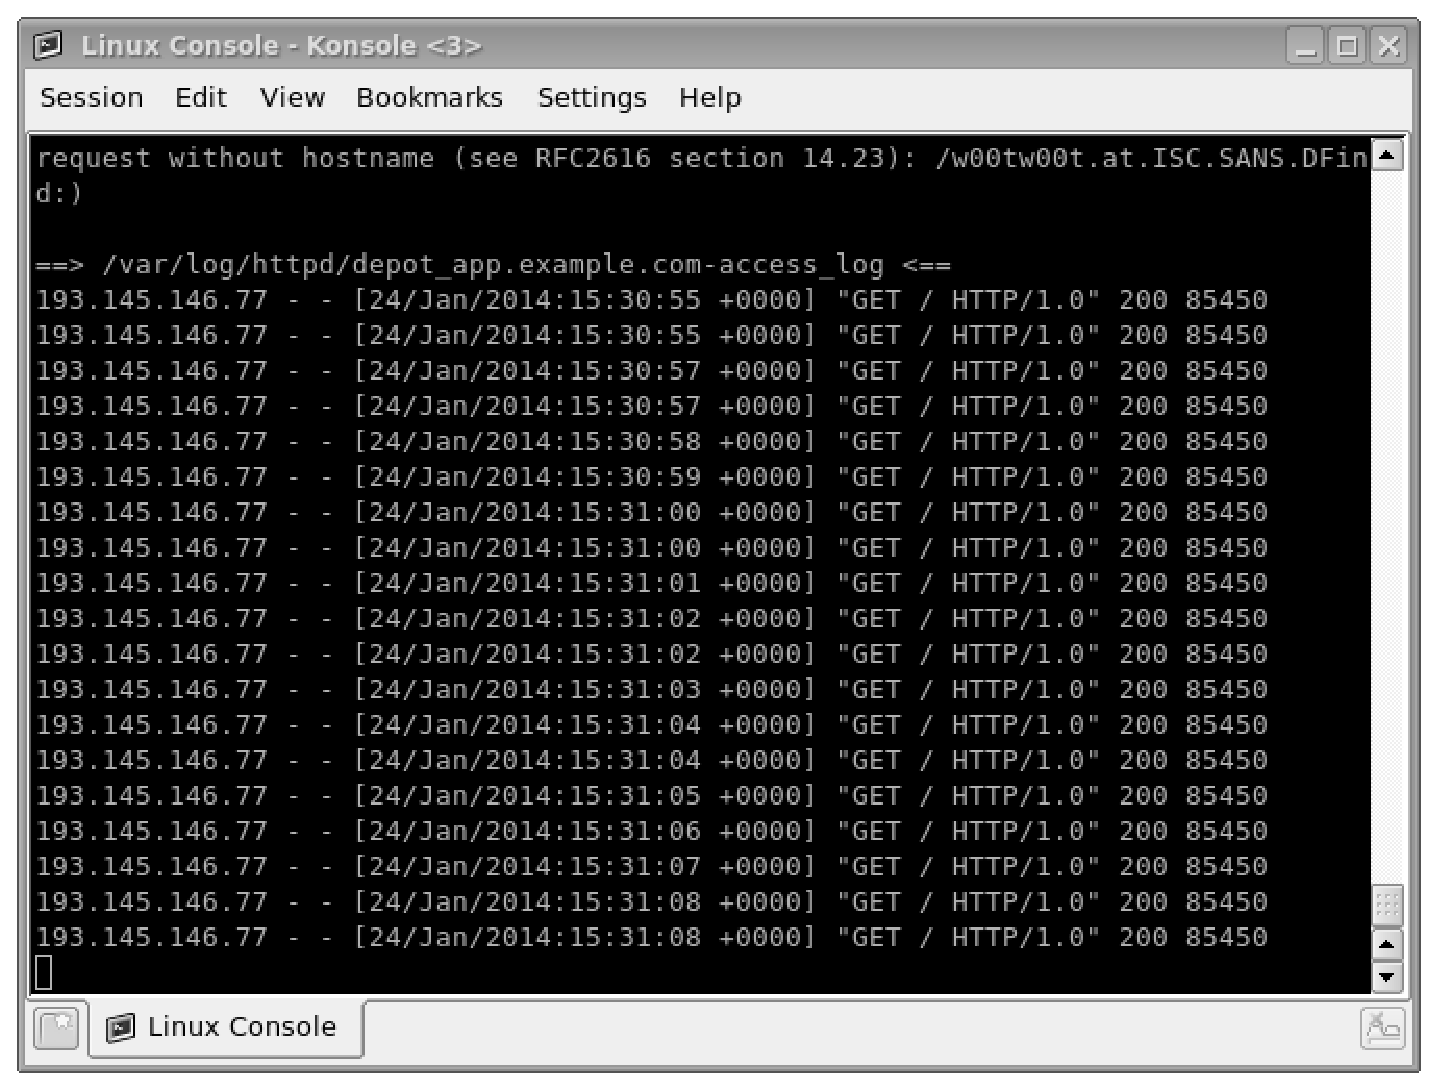
\includegraphics[scale=0.15]{logapache.eps}

\item Tail the Unicorn log files as \texttt{depot\_app} in \acrshort{ec2} in order to check Unicorn Server
\lstset{language=shell}
\begin{lstlisting}[escapechar=!]
$ tail -f log/production.log log/unicorn.std*
\end{lstlisting}
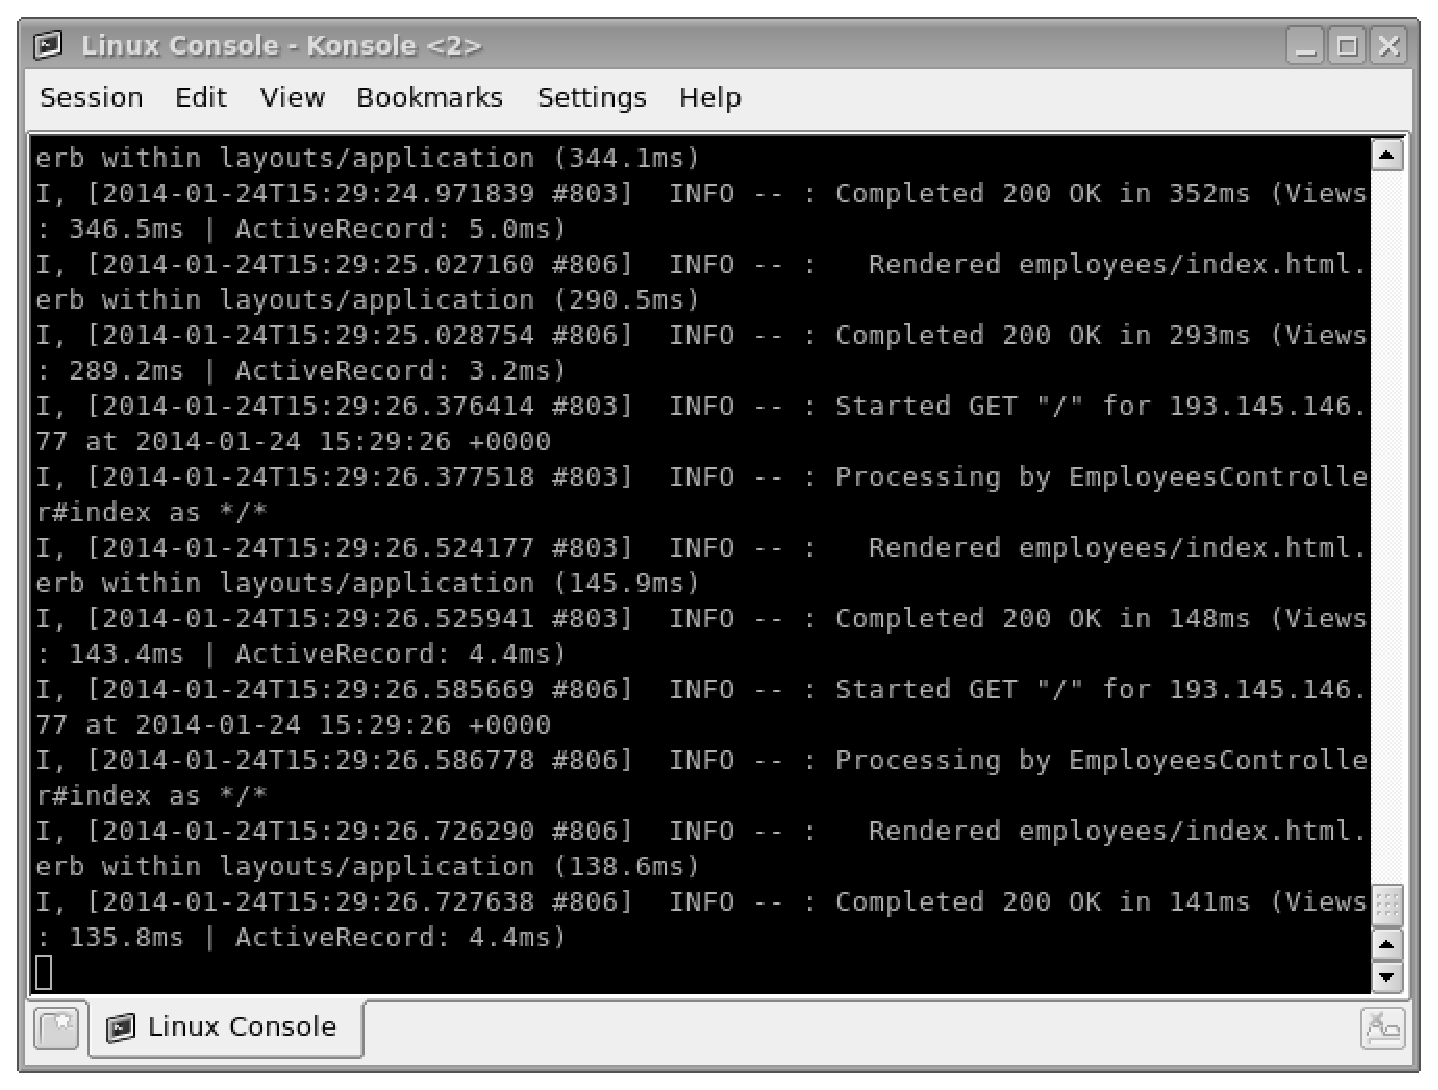
\includegraphics[scale=0.15]{lograils.eps}
}
\item Run JMeter (More info in \url{http://jmeter.apache.org/index.html}) and create a test plan


\begin{enumerate}
\item Right-click on the Test Plan node and choose \texttt{Añadir - Hilos (Usuarios) - Grupo de Hilos}
\item Configure the thread group with 120 threads, a ramp-up period of 360 seconds (6 minutes), and a loop count of 1
\item Right-click on the new Thread Group node and choose \texttt{Añadir - Muestreador - Petición HTTP}
\item Enter your elastic load balancer  name  ( omit the \texttt{http://} protocol prefix) and set port (80  should be fine)
\item Enter \texttt{``/''} for the path to retrieve the home page from the site
\item Right-click on the Test Pl an node once again. Add the following listener nodes: \texttt{Gráfico de resultados, Informe Agregado, and Generar Resumen de Resultados}

\end{enumerate}

\begin{center}
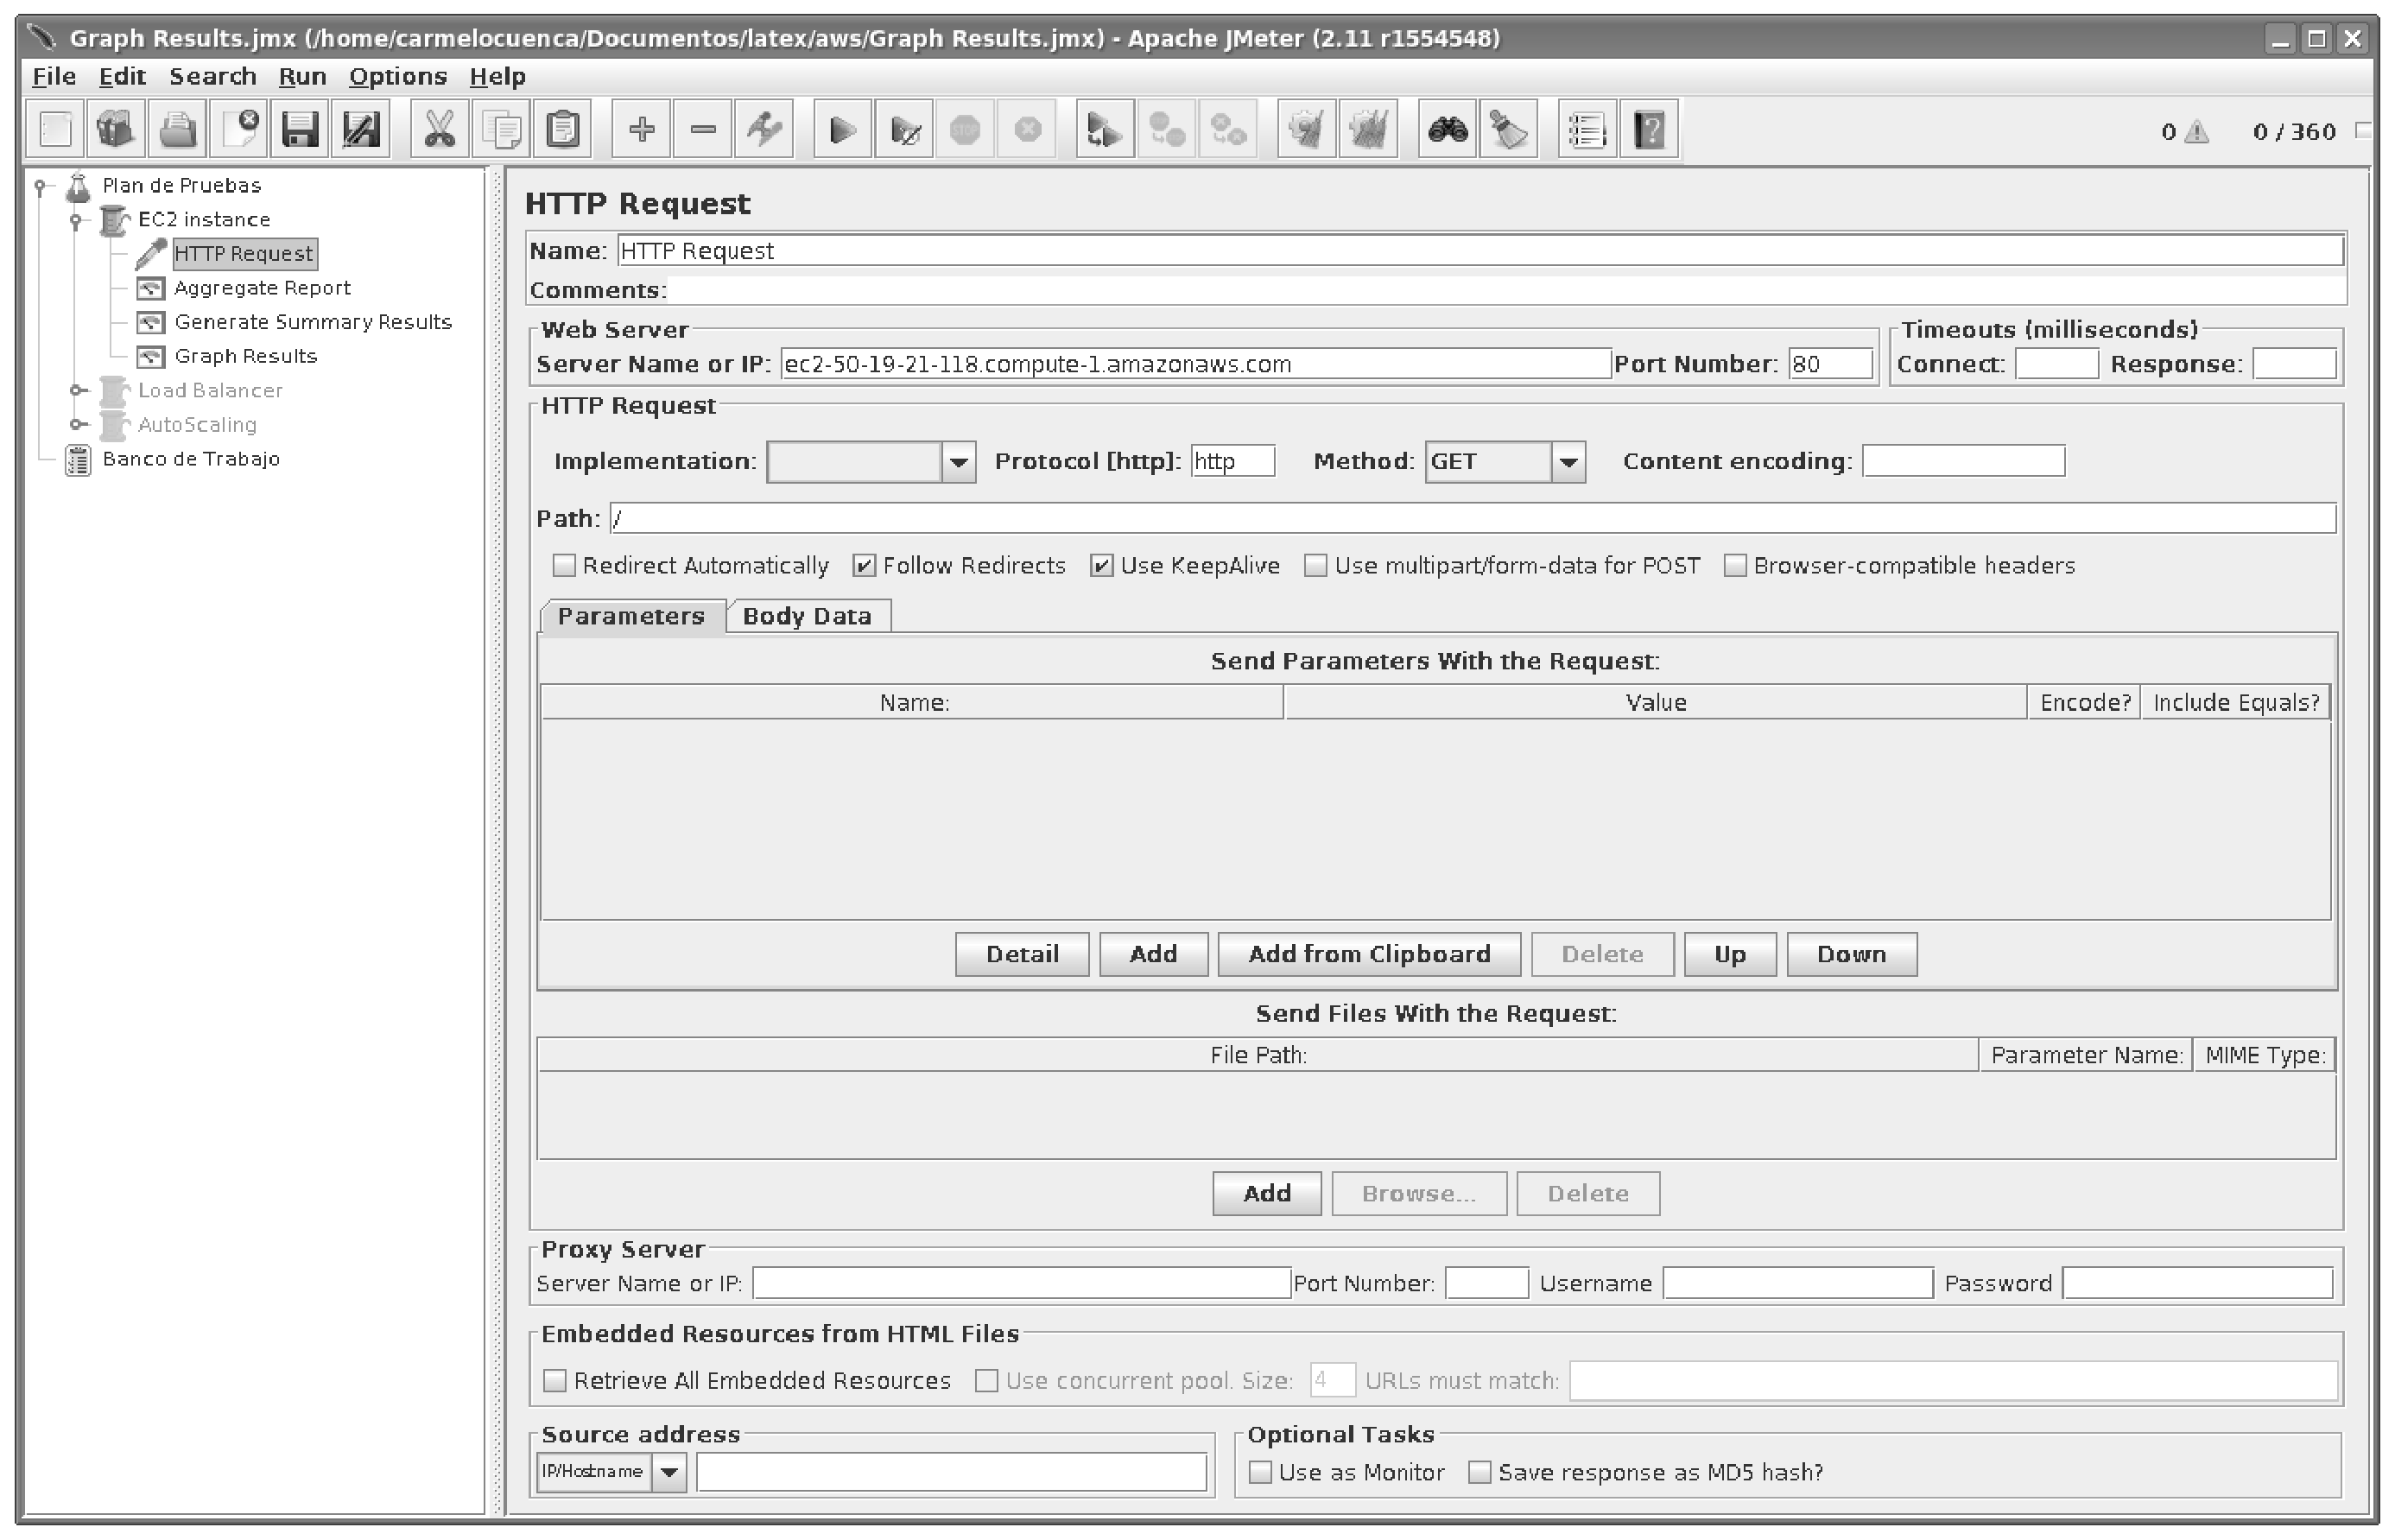
\includegraphics[scale=0.15]{plandeprueba.eps}
\end{center}
\begin{center}
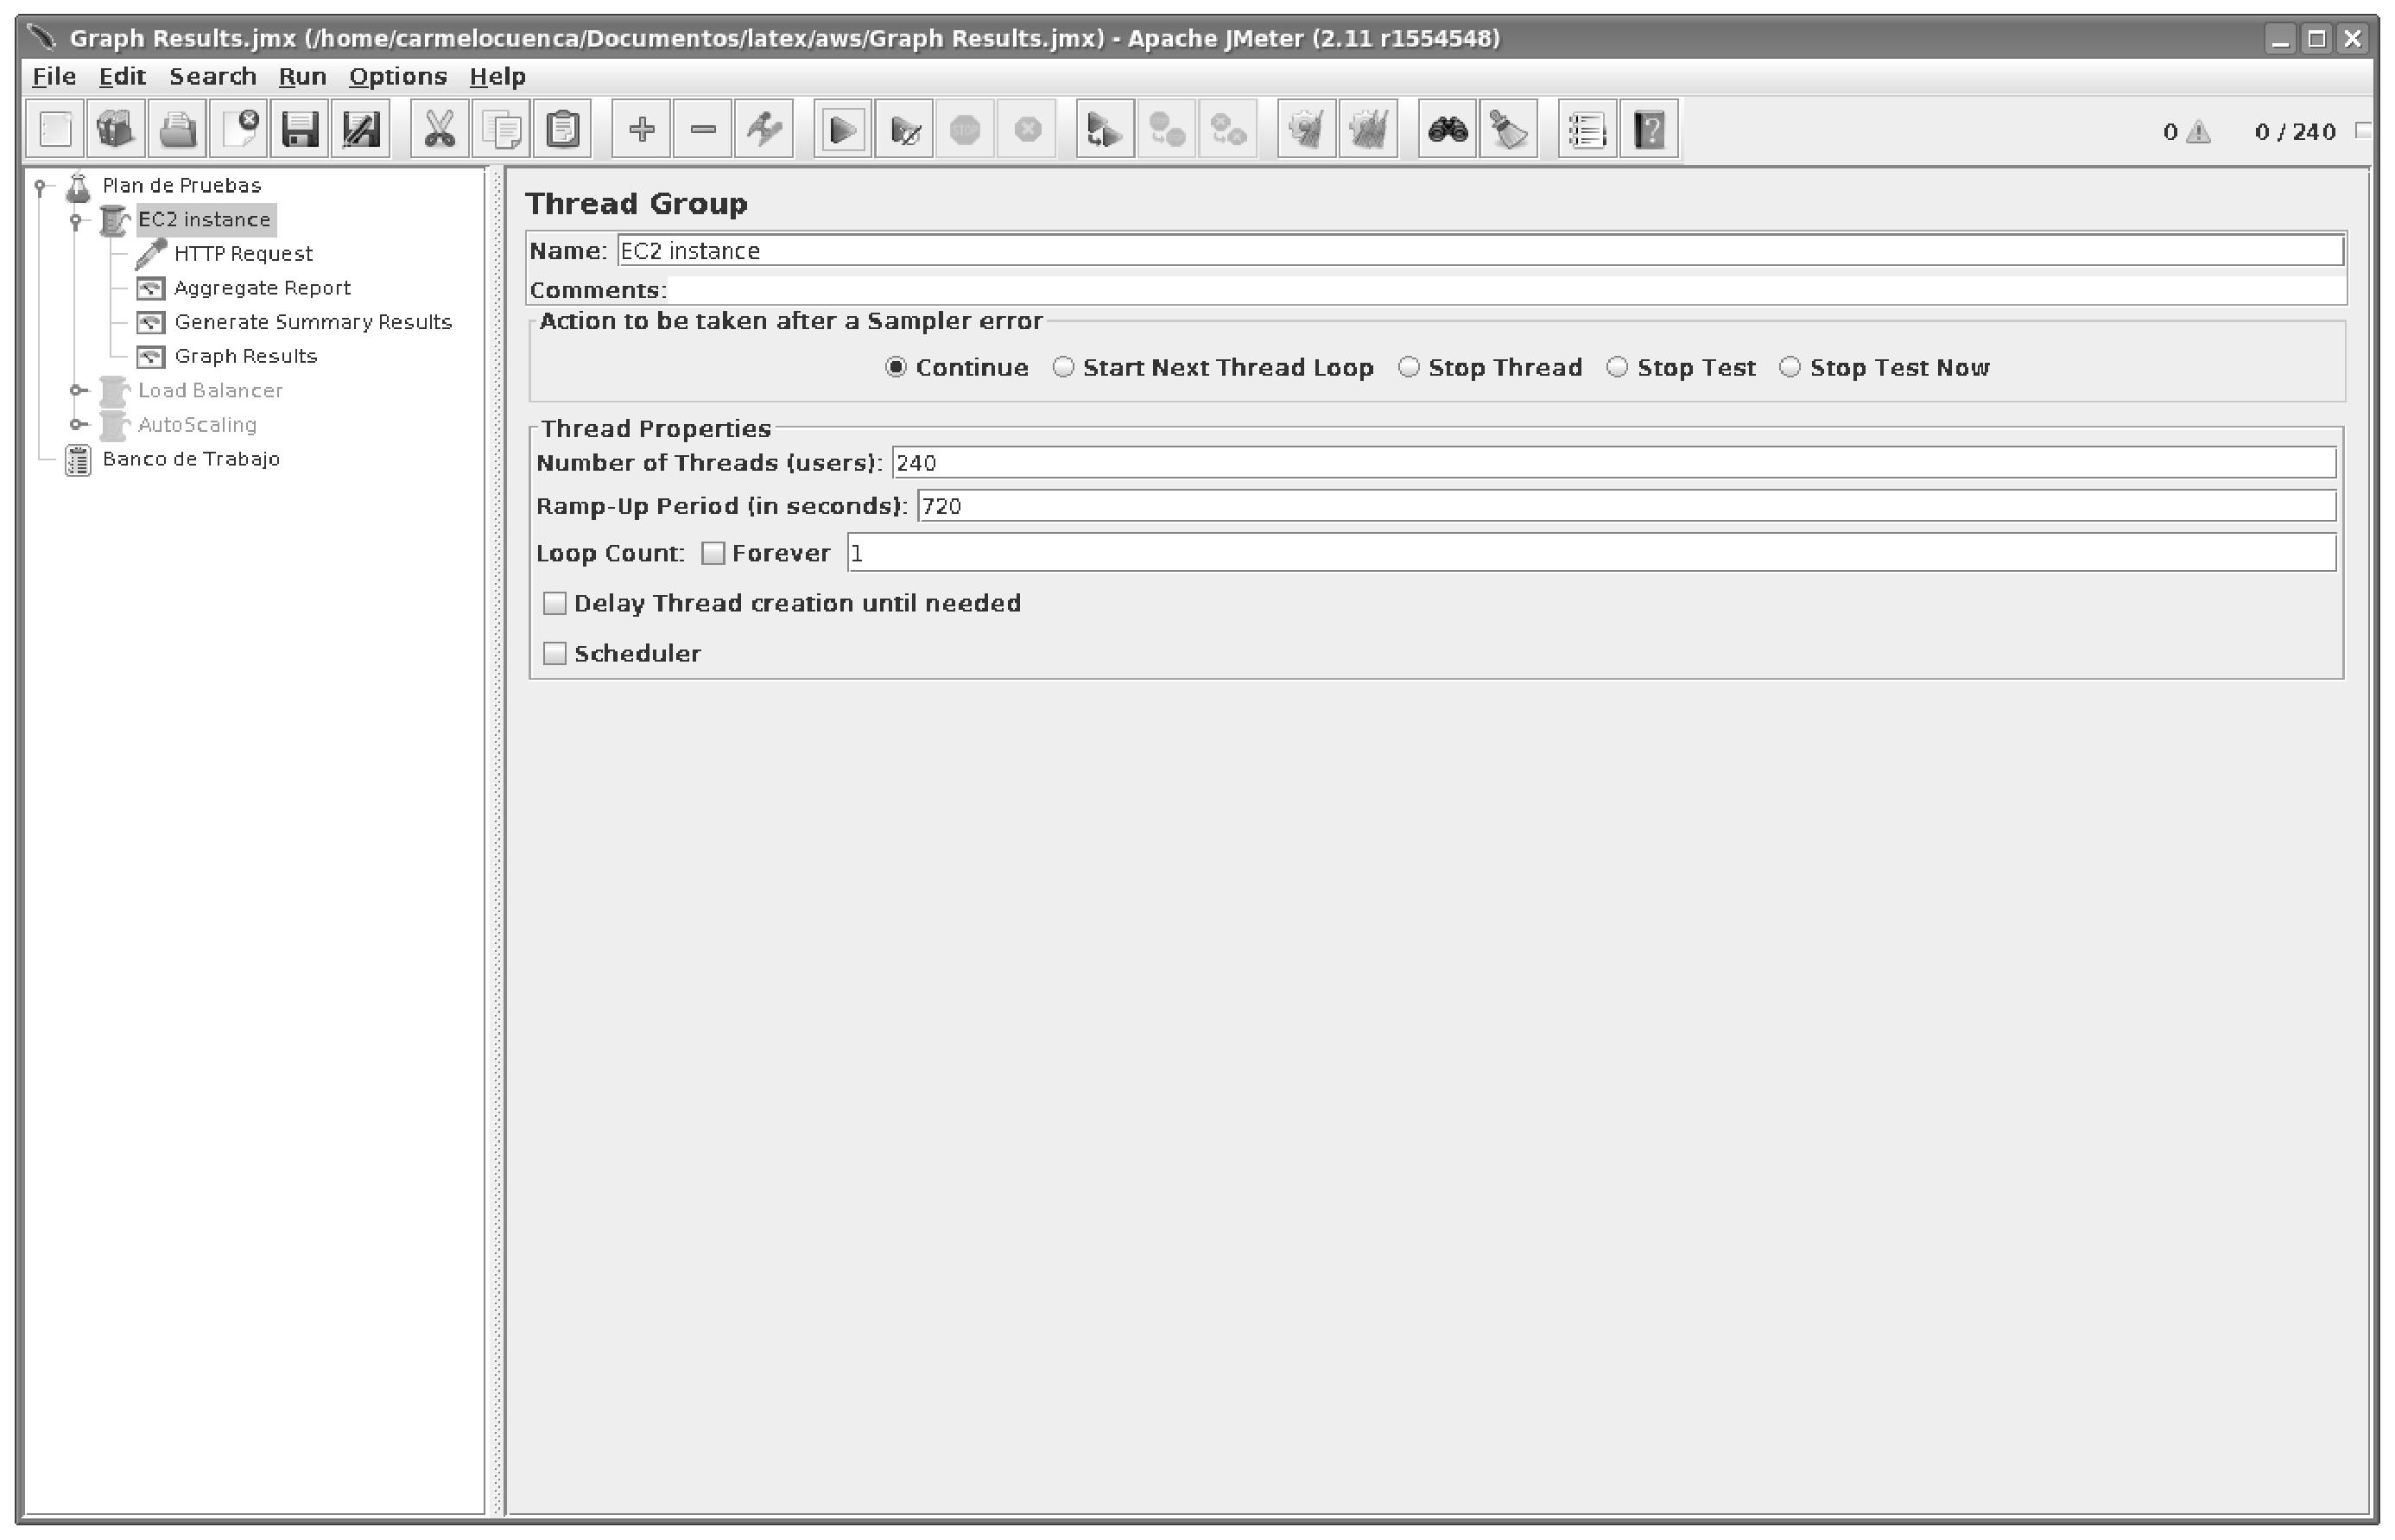
\includegraphics[scale=0.15]{plandeprueba1.eps}
\end{center}


\item Monitoring results and CloudWatch metrics in the ``Monitoring Tab''
\begin{center}
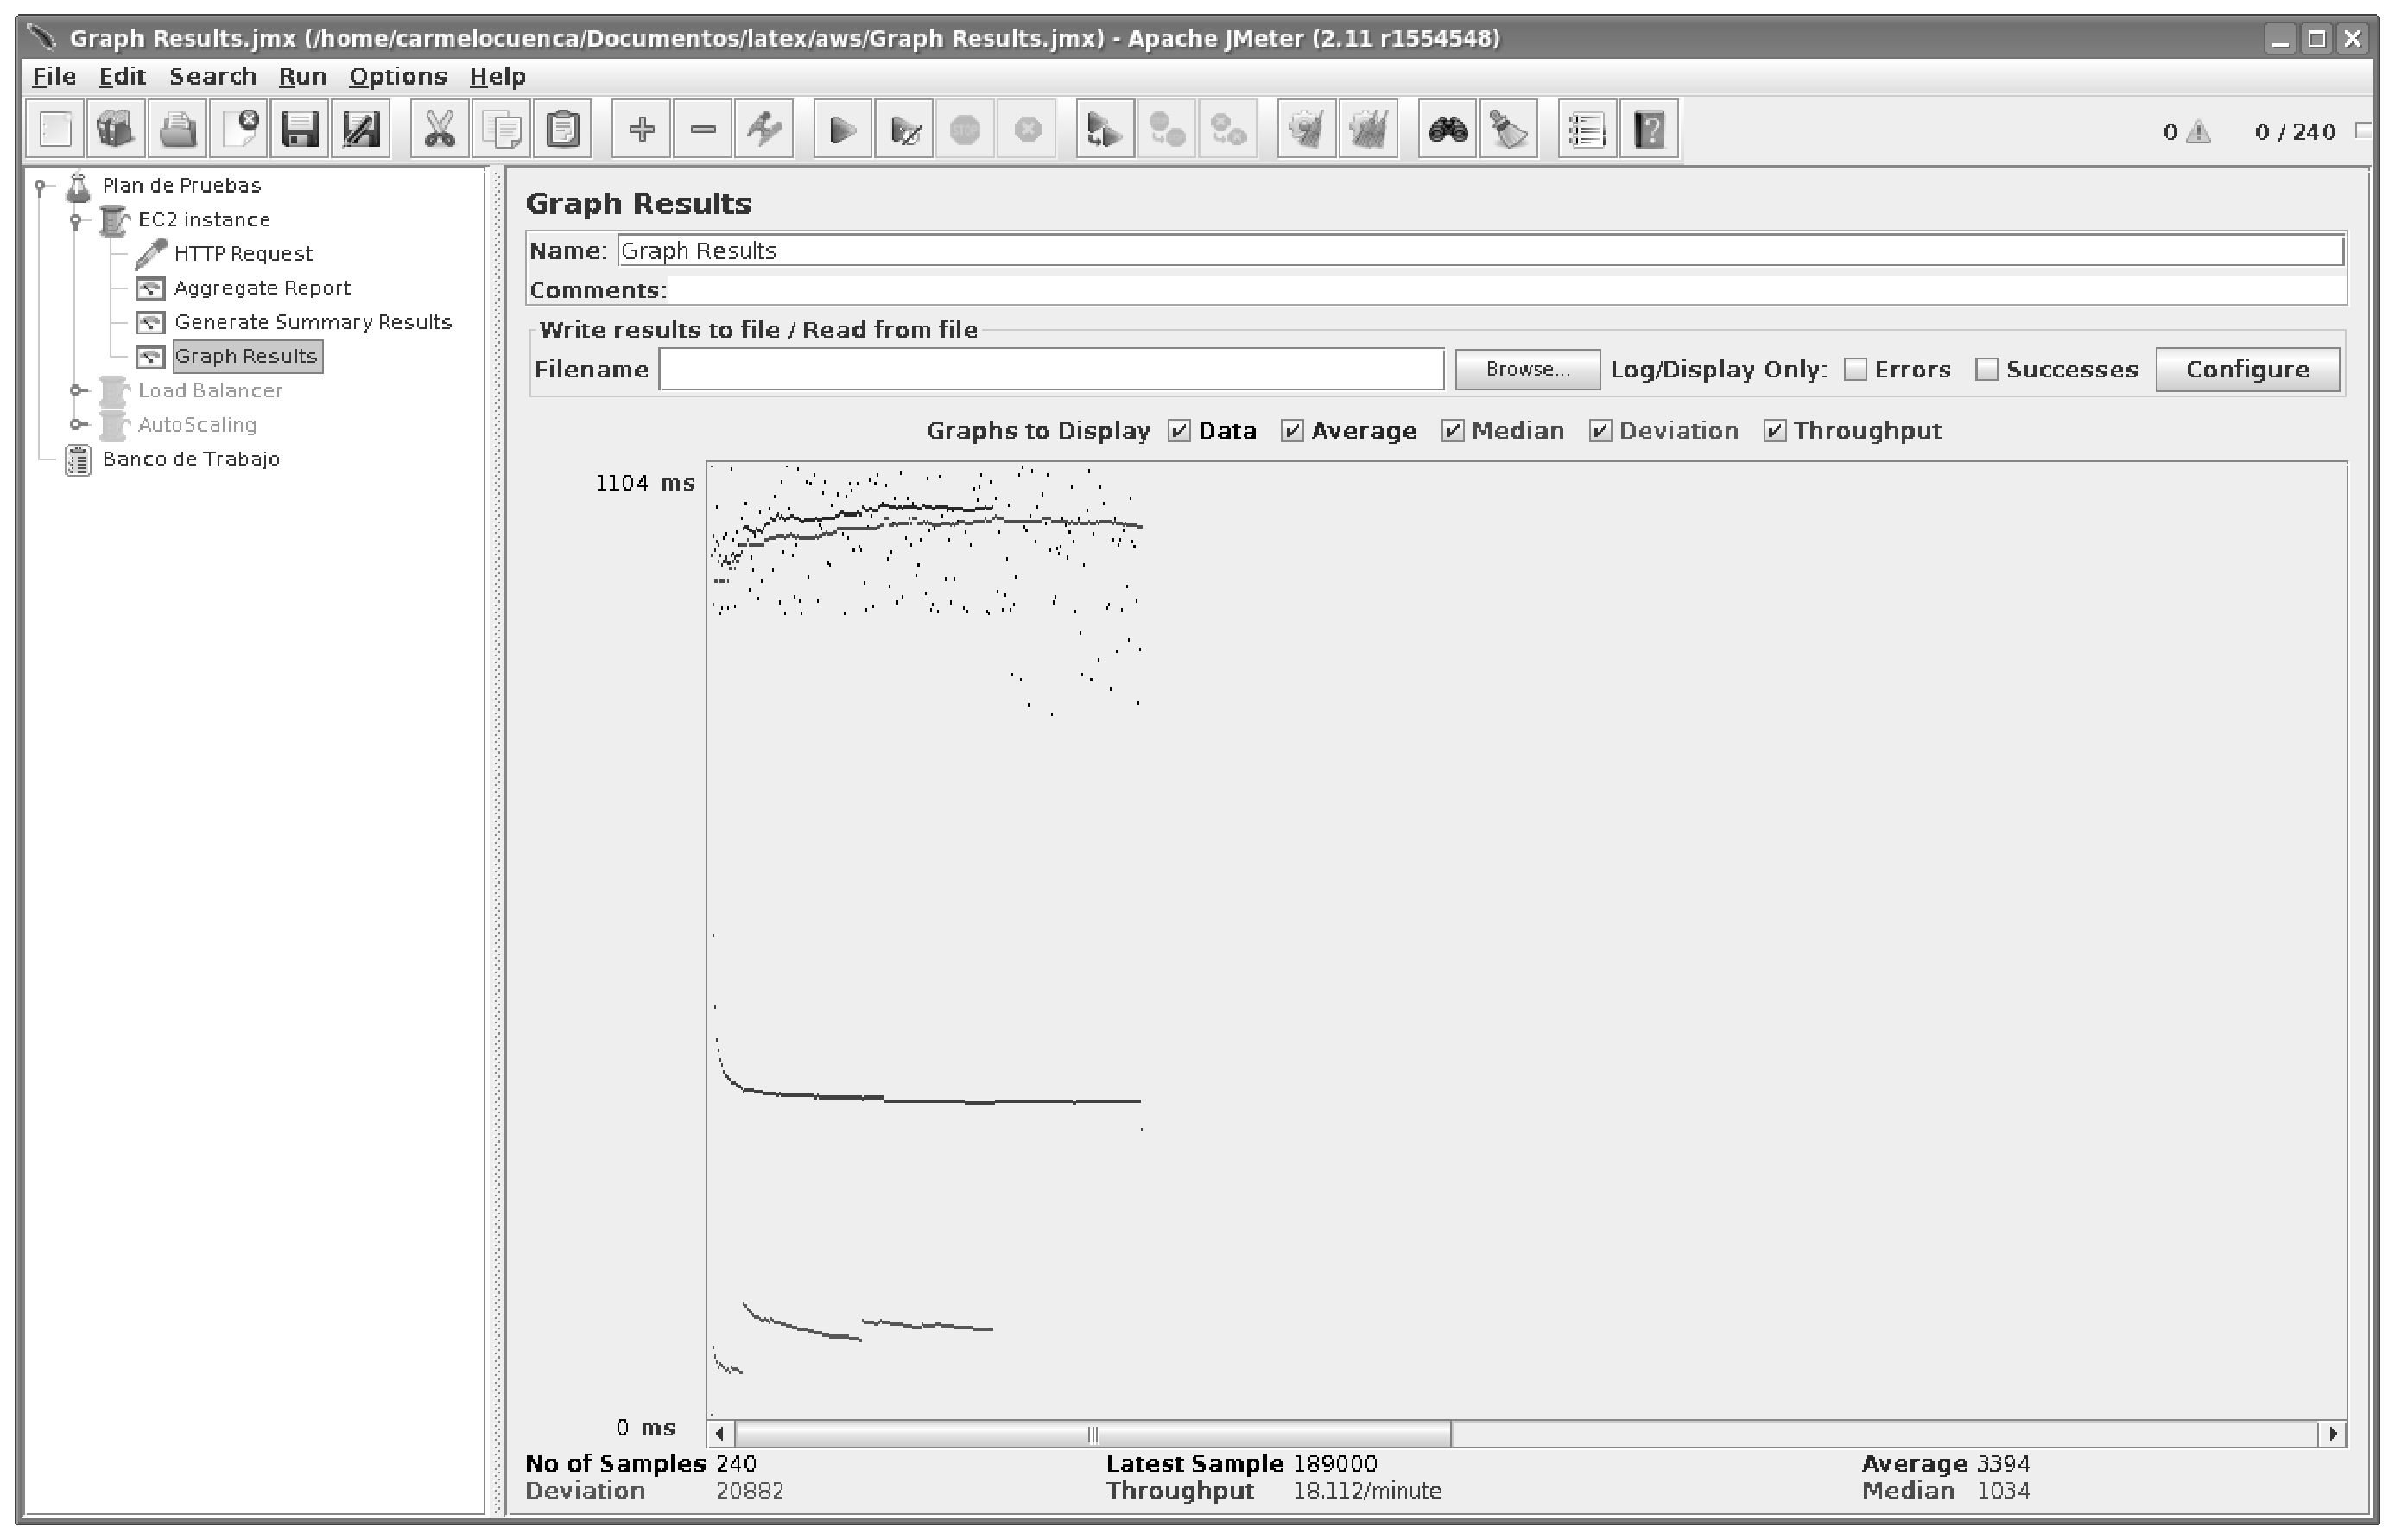
\includegraphics[scale=0.15]{plandeprueba2.eps}
\end{center}
\comment{
\begin{center}
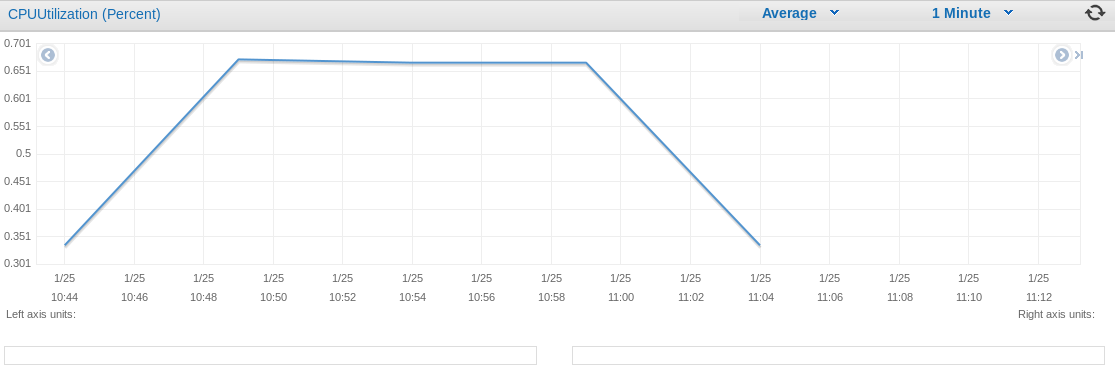
\includegraphics[scale=0.15]{cpuutilization.png}
\end{center}
}
\end{itemize}

\end{frame}

%%%%%%%%%%%%%%%%%%%%%%%%%%%%%%%%%%%%%%%%%%%%%%%%%%%%%%%%%%%%%%%%%%%%%%%%%%%%%%%%%%%%%%%%%%%%%%%%%%%%%%%%%%%%%%%%%%%%%%%%%%%%%%%%%%%%%%%%%%
\section{Homework}
\begin{frame}[fragile]
\frametitle{Homework}
\begin{itemize}
\item El próximo \texttt{dd/mm/aaaa} tendrá lugar a la hora \texttt{hh/mm/ss} el evento del año para nuestro ``site'' (venta de las entradas de la
``Gala Drag Queen'', lanzamiento de la versión beta del ``Grand Theft Auto'' o simplemente el anodino acceso a una plataforma ``Moodle'' de todos los alumnos simultaneamente a las \texttt{8:30} hora de la mañana al inicio de un día). 
Utiliza \acrshort{elb}, AutoScaling, CloudWatch para provisionar instancias para solventar ese pico horario. Comprueba el provisionamiento y la terminación de las instacias

\item Scale your favorite Content Management System (Joomla!, Drupal \dots) in Amazon
\end{itemize}
\end{frame}
%%%%%%%%%%%%%%%%%%%%%%%%%%%%%%%%%%%%%%%%%%%%%%%%%%%%%%%%%%%%%%%%%%%%%%%%%%%%%%%%%%%%%%%%%%%%%%%%%%%%%%%%%%%%%%%%%%%%%%%%%%%%%%%%%%%%%%%%%%

\end{document}

